% =====================================================================
%  Evolving Verifiers — NeurIPS Evaluations & Datasets (E&D) submission (anonymous)
%  v1.3 (677d): paper-merge batch. The 677b (clone-family-aware A5 split + cluster bootstrap)
%      and 677c (non-degenerate pools + five baselines + an executable evolution operator)
%      RESULTS ARE NOW FOLDED IN. No new experiments were run in 677d itself.
%      - A5 is now reported SIDE BY SIDE: +24.0pp full pool (k=4) and approx +7-12pp on the
%        degenerate-free pool (k<=3 significant; the k=|A|-1 zero is a set collision, 1/C(5,4));
%        clone-family re-splits leave the endpoint unchanged (+23.0 to +26.7pp) => template
%        leakage excluded; the family-level cluster bootstrap gives EFFECTIVE n ~133-140
%        (design effect ~4.2) and 1.78-2.10x wider intervals.
%      - New appendix paragraphs: "Clone-aware re-split and cluster bootstrap (677b)" and
%        "Non-degenerate pools, baselines and an executable operator (677c)"; the operator now
%        has an executable score function with its two disclosed collapses and a NON-significant
%        ablation (full vs frequency-only: +1.41pp, p=0.302, 3/14 tiers).
%      - The claim stays DIRECTIONAL ("evidence for the mechanism", never "FD beats Random").
%      - Main text held at 8 pages of content (References start on page 9) by compressing prose.
%  v1.2 (677a): framing revision + engineering cleanup. NO NEW EXPERIMENTS, NO NEW NUMBERS.
%      - VERSION OF RECORD: see research/latex/VERSION.md (single source of truth for
%        which artifact version every number in this paper comes from).
%      - 677a changes are *framing only*: (B) "verifier" is always an evidence-acquisition
%        apparatus, pass != semantic truth (new \S\ref{sec:threat} paragraph + first item of
%        \S\ref{sec:claim}); (C) the 38.4% blind-spot ratio is an instrument-boundary
%        statistic and is qualified at every occurrence; (D) Verifier Coverage 73.8% is a
%        descriptive census statistic -- the Clopper-Pearson CI was removed; (E) e-process
%        compressed to 2 sentences in the main text, full text in Appendix~\ref{app:eprocess}
%        and marked EXPLORATORY; (F) "74 real defects" -> "74 source-derived
%        reconstructions"; (H) engineering incident logs moved to Appendix~\ref{app:incidents}
%        so the main text carries findings, not project management.
%      - Numbers are identical to v1.1 (676m) except one *artifact-alignment* fix:
%        "15 of 70" high-blind-spot types -> "18 of 70" (677a) -> "13 of 34" (681:
%        label-normalized recompute from the repaired matrix; authoritative artifact
%        data/681_type_stats_normalized.json. Sample-level 38.4%/707/440 unchanged).
%  v1.1 (673c): red-team critique revisions + humanization. ALL NUMBERS IDENTICAL TO v1.0.
%  v1.0 (673a): all numbers synced to the authoritative numbers artifact (schema 672h).
%  Engine: tectonic (XeTeX) / pdflatex+bibtex.
%  Template: official neurips_2025.sty -- PLACEHOLDER. We target the NeurIPS 2027
%  Evaluations & Datasets (E&D) track (renamed from Datasets & Benchmarks in 2026).
%  The 2027 CFP is not published; this draft will migrate to the 2027 E&D style upon
%  release. Do NOT edit neurips_2025.sty (third-party file); the "Submitted to 39th
%  Conference ... (NeurIPS 2025)" footer it generates is a known placeholder artifact.
% =====================================================================
\documentclass{article}

\usepackage[dandb]{neurips_2025}   % Datasets & Benchmarks track; anonymous by default
\usepackage[utf8]{inputenc}
\usepackage[T1]{fontenc}
\usepackage{hyperref}
\usepackage{url}
\usepackage{booktabs}
\usepackage{amsfonts}
\usepackage{amsmath}
\usepackage{amssymb}
\usepackage{graphicx}
\usepackage{xcolor}
\usepackage{tikz}
\usepackage{pgfplots}
\pgfplotsset{compat=1.17}
\usetikzlibrary{arrows.meta,positioning,shapes.geometric,fit,backgrounds}

% placeholder for results pending the baseline batch (kept visible on purpose)
\newcommand{\TODO}[1]{\textcolor{red}{\textbf{[TODO: #1]}}}
\newcommand{\cmark}{\textcolor{green!60!black}{\checkmark}}

\title{Evolving Verifiers: Failure-Driven Evidence\\ Acquisition with Auditable Provenance}

\author{%
  Ran Liao \\
  School of Artificial Intelligence and Big Data \\
  Hefei University, Hefei, Anhui, China \\
  \texttt{1026708211@qq.com} \\
}

\begin{document}
\maketitle

\begin{abstract}
At near-zero generation cost, the bottleneck moves to evolving the evidence-acquisition apparatus.
Existing benchmarks evolve the items; we evolve the verifier's evidence-acquisition capability,
under an externally interruptible audit discipline. Throughout, ``verifier'' means an
evidence-acquisition apparatus, not an oracle of truth: a pass means no acquired evidence
contradicts the assertion within the capability boundary, not semantic correctness. We present
\textbf{Queyi}: conclusion--evidence--recomputation bound into a chain, the verifier's own failures
the only legal input to evolution. Objects are executable C++ assertions judged by four-state
verdicts; credibility: a forced provenance/scope split and a kernel-independent
reconciler. Queyi has 67 rules, 42 real cards (31 with evidence anchors; Verifier Coverage
73.8\%), a 452-event ledger and Merkle roots over 5 directories. On the same
samples, expanded holdout recall is 82.9\% (34/41), 81.0\% (17/21) strictly pre-reveal
blind; corpus measurable recall is 62.5\% (40/64), versus a static caliber arm 2.4\%/17.2\%
($\Delta$ +80.5/+45.3pp) and an instrument-level random proxy 9.8\%/21.9\% ($\Delta$
+73.2/+40.6pp); exact McNemar $p\le3.0\times10^{-8}$. Limitations: headline numbers depend on one
WSL environment; $n{=}41/64$ is small; only 21 samples are strictly blind; the
static arm is a caliber re-binning, the random arm a proxy. We claim auditability plus on-sample
significance, not superiority over real static detectors. The A5 budget-matched control runs at
full scale ($n{=}566$): FD 54.6\% vs.\ Random 30.6\% (+24.0pp full pool, $p{=}2.3\times10^{-41}$), vs.\
Static 24.7\% (+29.9pp); excluding degenerate assets Random draws the same four at $k{=}4$, while
$k\le3$ keeps +7.4--+11.3pp (effective $n\approx133$--$140$ after clone-family re-splitting).
A5 isolates ``do not fund assets that cannot inform,'' not
``a smarter ranking''. Labels have AI self-consistency only ($\kappa{=}0.77$).
\end{abstract}

% =====================================================================
\section{Introduction}
\label{sec:intro}
% =====================================================================
\paragraph{The problem: generation is easy, verification is not.}
When LMs generate knowledge in bulk, the bottleneck shifts from ``generating correct
knowledge'' to \emph{evolving verifiers that keep pace with generation}: memorization and
contamination wear out a fixed yardstick, and the very samples a verifier has graded domesticate it.
The question is therefore not ``how do we verify this batch of knowledge,'' but ``how does a verifier
evolve without grading its own homework, with every step independently auditable.''
We ground this paradigm claim in an executable setting: an LLM can emit
thousands of C++ technical assertions in minutes, and they are \emph{numerous} (manual review does
not scale), \emph{plausible} (syntax and tone look right), and \emph{quietly wrong} (errors surface
only under a specific flag, compiler, or platform). The asymmetry---\textbf{generation cost tends to
zero, verification cost does not}---is the starting point of this work. Executable evaluation of
generated code has precedent~\cite{chen2021humaneval}; our question differs---not whether code
passes tests, but whether a knowledge claim is supported by recomputable evidence.

\paragraph{The object of study is the measuring stick, not the score.}
The instrument that produces a score is itself subject to Goodhartization---it drifts, is
re-calibrated, silently breaks---and that drift is \emph{measurable}. We therefore treat the
evaluation apparatus as a \textbf{first-class scientific object}: publish its capability boundary,
require every rate to carry the caliber that produced it, and let the apparatus's own failures be
the only legal input to its evolution~\cite{zhang2026whogrades}. Our findings are of two kinds---
numbers about C++ assertions, and \emph{numbers about the instrument}---and the second kind is the
one we argue generalizes.

\paragraph{Motivation 1: high scores $\neq$ real ability.}
SWE-bench turned ``fix real GitHub issues'' into a yardstick~\cite{jimenez2024swebench}, but
follow-up work is systematically negative: gains on SWE-bench-Verified are partly \emph{memory
rather than reasoning} (76\% file location inside the repo vs 53\% outside~\cite{liang2025illusion};
$3\times$ higher than on two sibling benchmarks~\cite{prathifkumar2025verified}), and SWE-MERA
reports 32.67\% of successful patches involving solution leakage and 31.08\% passing on insufficient
tests~\cite{adamenko2025swemera}. \emph{Implication:} a verifier tested on its own data reproduces
this failure, so we choose \textbf{external samples first}, \textbf{irreversible blinding},
\textbf{layered reporting}.

\paragraph{Motivation 2: AI-text detection answers the wrong question.}
DetectGPT~\cite{mitchell2023detectgpt} and watermarking~\cite{kirchenbauer2023watermark} answer
``was this text written by an AI?'', fragile to paraphrase~\cite{sadasivan2023canai}. More
fundamentally, \textbf{provenance and truth are independent questions}. \emph{Implication:} we do
not detect provenance; we \textbf{test assertions} (compile, warn, sanitize, cross-compiler and
cross-optimization diff).

\paragraph{Contributions.}
(1)~\textbf{A definition and three checkable properties of failure-driven verifier evolution} (\S\ref{sec:method}): evolution
is an operator $E(\mathcal{C}_t, F_t)$ acting on the evidence-acquisition capability
$\mathcal{C}_t$ and driven \emph{only} by registered failures $F_t$, with three checkable
properties---\emph{monotonicity} (evolution never removes evidence capability), \emph{minimality}
(every new rule must trace to a registered failure), and \emph{auditability} (each step leaves the
chain \emph{failure} $\to$ \emph{rule} $\to$ \emph{re-test}).
(2)~\textbf{A caliber analysis of the four-state verdict} (\S\ref{sec:method}):
each verdict is a Belnap four-valued state $(\mathrm{support},\mathrm{refutation})$ over registered
evidence---$\texttt{pass}=(1,0)$, $\texttt{fail}=(0,1)$, $\texttt{unknown}=(0,0)$,
$\texttt{contradict}=(1,1)$~\cite{belnap1977useful}---while \emph{detector availability} is
\emph{separate metadata}, not a coordinate. Merging \texttt{unknown} into
\texttt{miss} pollutes the denominator; into \texttt{pass} it manufactures false confidence. The
primary estimand therefore conditions on measurable samples (catch $+$ miss), with alternative
denominators reported separately.
(3)~\textbf{Three conditions for auditability} (\S\ref{sec:method}): \emph{origin
traceability} (every verdict decomposes into rule $\times$ evidence), \emph{state
reproducibility} (a third party rebuilds verdict-time inputs from on-disk artifacts), and
\emph{tamper detectability} (any change to a controlled directory moves the Merkle root).
A runnable instantiation (67 rules, a 452-event ledger, five controlled directories) realizes these
\emph{for the current state}, with \emph{partial} historical pinning. \textbf{We give no theorems}:
the three properties are design constraints not yet verified rule-by-rule over the 67 rules, and the
``caliber analysis'' is qualitative---we claim no novelty in the four-state encoding.

\paragraph{What we do \emph{not} claim.} Not a better textbook, a stronger detector, or a formal
proof; and not that ``the verifier got stronger'' unless measured on the \emph{same external
samples under the same caliber} (\S\ref{sec:exp}, Fig.~\ref{fig:evolution}).

% =====================================================================
\section{Related Work}
\label{sec:related}
% =====================================================================
We compress prior work into five lines (two further directions, and an eight-direction table, are in
Appendix~\ref{app:related}). All comparisons are \emph{positional and qualitative}, not empirical
claims about those systems.

\paragraph{(1) Self-evolving / contamination-resistant benchmarks (they evolve the \emph{items}).}
Benchmark Self-Evolving~\cite{wang2024benchmarkevolving}, ArenaBencher~\cite{liu2025arenabencher},
SWE-bench-Live~\cite{zhang2025swebenchlive}, DynaBench~\cite{kiela2021dynabench} and
LiveBench~\cite{white2024livebench} all fight ``the model memorized the items'', but they evolve
the \emph{object under test}; who judges, and whether the judgment is right, stays a fixed oracle.

\paragraph{(2) Mutation-guided LLM test generation (the closest engineering form).}
ACH~\cite{foster2025ach} and MUTGEN~\cite{wang2025mutgen} turn mutation testing from an
\emph{evaluation} device into a \emph{generation} device; Cleverest~\cite{liu2025cleverest} does
just-in-time regression test generation. We \emph{reuse} the mutation-feedback idea as an internal
self-justification layer, but we \emph{refuse} to treat mutation score as a defect-detection rate.

\paragraph{(3) Self-verification / LLM-as-a-judge (partly adopted, partly rejected).}
LLM-as-a-judge~\cite{zheng2023judging} is practical and scalable, but we use LLMs only to
\emph{propose candidates} and keep the \emph{judgment} fully programmatic; model-based
verifiers~\cite{kwok2026llmverifier} keep the judge inside the model, against which our
shared-failure-domain objection stands (\S\ref{sec:exp}, E7). (Formal verification, program
analysis and measurement governance: Appendix~\ref{app:related}.)

\paragraph{(4) Trained fact-checking models (the nearest neighbor where the \emph{judge} itself evolves).}
Trained fact-checkers~\cite{tang2024minicheck} evolve \emph{the judge} itself, so auditability
reduces to trusting model behaviour---complementary to us (\S\ref{app:related}).
\paragraph{(5) Closest 2026 work (metric evolution and self-evolving verification).}
Full text in \S\ref{app:related} (Table~\ref{tab:neighbours}). \emph{Who Grades the
Grader?}~\cite{zhang2026whogrades} evolves the evaluation \emph{metric} itself against Goodhart
drift---the closest analogue to our anti-Goodhart discipline, but its evolved object is a metric,
not a verifier's evidence-acquisition capability; \emph{Self-Evolving Agents with Anytime-Valid
Certificates}~\cite{sengupta2026anytimevalid} is an agent framework, not a C++ assertion protocol.
\textbf{We do not claim to be the first to evolve an evaluator}: our claim concerns the evolved
object and the recomputable \emph{failure}$\to$\emph{rule}$\to$\emph{re-test} chain.
Table~\ref{tab:positioning} (Appendix~\ref{app:tables}) positions eight works along five dimensions.


% =====================================================================
\section{Problem Definition and Threat Model}
\label{sec:threat}
% =====================================================================
\paragraph{Formalization.}
A \emph{knowledge assertion} $a$ is a decidable statement plus a \emph{boundary triple}
$\langle D, P, F\rangle$ (input domain, preconditions, failure conditions). \emph{Evidence} $e$ is
a replayable observation (compiler version $+$ command $+$ optimization level $+$ output $+$
content-addressed hash). A \emph{verdict} is $v\in\{\texttt{pass},\texttt{fail},\texttt{unknown},
\texttt{contradict}\}$; \emph{verification capability} $\mathcal{C}$ is the set of available
evidence-acquisition means. Our goal is \textbf{not} to maximize $\Pr[v{=}\texttt{pass}]$ but to
maximize agreement with ground truth \emph{without disguising \texttt{unknown} as \texttt{pass}}.

\paragraph{Why four states.} ``Detector unavailable'' and ``detector says fine'' are different
knowledge states (Fig.~\ref{fig:belnap}, Belnap's four-valued
logic~\cite{belnap1977useful}). Recording \texttt{unknown} as \texttt{miss} understates
capability; as \texttt{pass} it manufactures a \emph{false pass}; recording \texttt{miss} as
\texttt{unknown} hides a capability gap. Hence the \textbf{denominator is
$\text{catch}+\text{miss}$ (measurable samples)}, \texttt{unknown} and \texttt{not\_error} are
reported separately, and the caliber lives in the artifact, not in prose.

\begin{figure}[t]
\centering
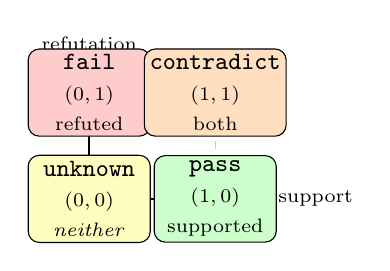
\begin{tikzpicture}[font=\small, x=1.6cm, y=1.35cm]
  \draw[->, thick] (-0.22,0) -- (1.42,0) node[right, font=\scriptsize] {support};
  \draw[->, thick] (0,-0.22) -- (0,1.30) node[above, font=\scriptsize] {refutation};
  \draw[gray!40, dashed] (1,0) -- (1,1) -- (0,1);
  \node[draw, rounded corners, fill=yellow!25, align=center, inner sep=2pt, minimum width=1.55cm]
    at (0,0) {\texttt{unknown}\\\scriptsize$(0,0)$\\\scriptsize\emph{neither}};
  \node[draw, rounded corners, fill=green!20, align=center, inner sep=2pt, minimum width=1.55cm]
    at (1,0) {\texttt{pass}\\\scriptsize$(1,0)$\\\scriptsize supported};
  \node[draw, rounded corners, fill=red!20, align=center, inner sep=2pt, minimum width=1.55cm]
    at (0,1) {\texttt{fail}\\\scriptsize$(0,1)$\\\scriptsize refuted};
  \node[draw, rounded corners, fill=orange!25, align=center, inner sep=2pt, minimum width=1.55cm]
    at (1,1) {\texttt{contradict}\\\scriptsize$(1,1)$\\\scriptsize both};
\end{tikzpicture}
\caption{Every verdict is a Belnap state $(\mathrm{support},\mathrm{refutation})$ over
\emph{registered evidence}: \texttt{pass}$=(1,0)$, \texttt{fail}$=(0,1)$, \texttt{unknown}$=(0,0)$,
\texttt{contradict}$=(1,1)$. \textbf{Detector availability is separate per-item metadata, not a
coordinate of this plane}: \texttt{unknown} means ``not registered either way'', never ``no detector
exists''.}
\label{fig:belnap}
\end{figure}

\paragraph{Terminology: what ``verifier'' means here.}
\label{sec:terminology}
We use ``verifier'' in the \textbf{evidence-acquisition} sense. A verifier \emph{acquires
reproducible evidence} about an assertion and records the Belnap state induced by it; it does
\emph{not} adjudicate semantic truth. \textbf{Verification} $=$ actively searching for evidence
that supports or refutes an assertion within a capability boundary $\mathcal{C}$;
\textbf{truth} $=$ semantic correctness, which we never claim to establish. A \texttt{pass} means
\emph{no acquired evidence contradicts the assertion}---not that it is true, and nothing about
classes outside the boundary (on our corpus \textbf{38.4\%} of samples are invisible to our
eight-asset instrument; \S\ref{sec:validity}, Appendix~\ref{app:blindspot}). A \texttt{miss} means
\emph{no refuting evidence was acquired}, not that the assertion holds.

\paragraph{Nineteen threats (T1--T19).}
Table~\ref{tab:threats} (Appendix~\ref{app:tables}) lists all nineteen with mitigations and
residuals; \S\ref{sec:validity} quantifies them under the standard validity
layers~\cite{shadish2002experimental}. The four bearing most on our claims are \textbf{T8} (budget
selection bias), \textbf{T13} (peeking), \textbf{T15} (untrusted LLM channel) and \textbf{T16}
(small-sample poisoning); the A0--A5 ablations and the e-process protocol (\S\ref{sec:method}) exist
to bound their residuals.


\paragraph{Three focus threats.}
\textbf{(a) Construct: a \texttt{catch} is evidence, not truth.} Switching the pipeline from
single- to dual-flag (\texttt{-O0}+\texttt{-O2}) moved recall \textbf{66.7\%$\to$87.5\% with the
detector unchanged}---\emph{the caliber changed, not the capability}. \textbf{(b) Meta-Goodhart:}
with no external reference the score can rise by changing the caliber or the denominator, and a
reported rate can be \emph{hollow}---produced by a caliber change never re-run, so it appears in the
paper but in no artifact while an automated \texttt{--check} on registered fields stays green:
\textbf{caliber drift is not self-announcing} (Appendix~\ref{app:incidents}). \textbf{(c)
Contamination:} leakage (T3), shared-criterion labeling (an upper bound, $F_1{=}1.0$), unblinded
expansion. Three further threats are registered: \textbf{T17} (single-annotator labels),
\textbf{T18} (public rules invite evasion), \textbf{T19} (three samples no sanitizer sees---%
\texttt{h46}, \texttt{h59}, \texttt{h60}---are both capability gaps and attack surface); full
statements in Appendix~\ref{app:humanize}.

% =====================================================================
\section{Method}
\label{sec:method}
% =====================================================================
\begin{figure}[t]
\centering
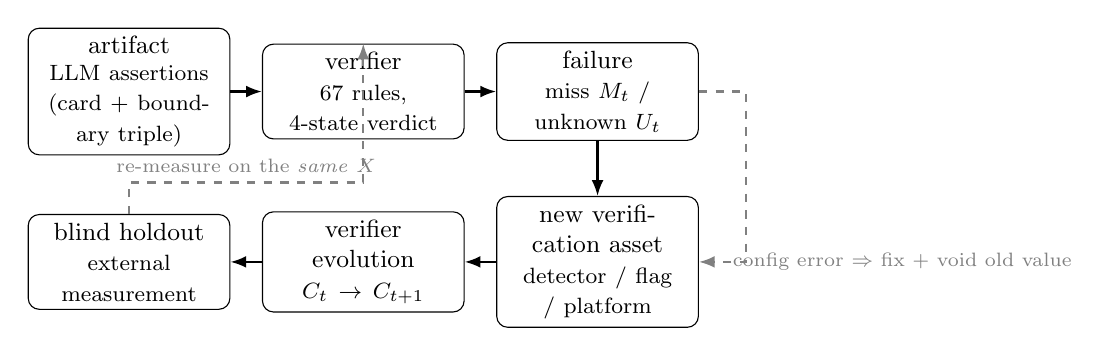
\begin{tikzpicture}[
  font=\small,
  box/.style={draw, rounded corners, align=center, inner sep=3pt, minimum height=9mm, text width=2.35cm},
  arr/.style={-{Latex[length=2mm]}, thick},
  fb/.style={-{Latex[length=2mm]}, dashed, thick, gray}
]
\node[box] (a) {artifact\\\footnotesize LLM assertions\\\footnotesize (card + boundary triple)};
\node[box, right=4mm of a] (b) {verifier\\\footnotesize 67 rules, 4-state verdict};
\node[box, right=4mm of b] (c) {failure\\\footnotesize miss $M_t$ / unknown $U_t$};
\node[box, below=7mm of c] (d) {new verification asset\\\footnotesize detector / flag / platform};
\node[box, left=4mm of d] (e) {verifier evolution\\\footnotesize $C_t \to C_{t+1}$};
\node[box, left=4mm of e] (f) {blind holdout\\\footnotesize external measurement};
\draw[arr] (a)--(b);
\draw[arr] (b)--(c);
\draw[arr] (c)--(d);
\draw[arr] (d)--(e);
\draw[arr] (e)--(f);
\draw[fb] (f.north) -- ++(0,4mm) -| node[pos=0.25, above, font=\scriptsize]{re-measure on the \emph{same} $X$} (b.north);
\draw[fb] (c.east) -- ++(6mm,0) |- node[pos=0.75, right, font=\scriptsize, align=left]{config error $\Rightarrow$ fix + void old value} (d.east);
\end{tikzpicture}
\caption{The failure-driven verification loop. Solid arrows form the main cycle; dashed arrows
are re-measurement and caliber correction. Tools: the rule engine (67 rules, four states), the
kernel-independent meta-state reconciler, and the counterfactual operator.}
\label{fig:loop}
\end{figure}

\paragraph{Architecture (summary; full in Appendix~\ref{app:formal}).}
\texttt{artifact}$\to$\texttt{verifier}$\to$\texttt{verdict}$\to$\texttt{ledger}
(Fig.~\ref{fig:loop}): knowledge cards with a boundary triple; \textbf{67} rules producing
four-state verdicts; content-addressed evidence per compile/run (\textbf{28} cards at L1,
\textbf{28} double-compiler confirmed, \textbf{147} real compilations); and a \textbf{452}-event
append-only ledger under a zero-change red line.

\paragraph{Four-state verdict.}
The four states are drawn in Fig.~\ref{fig:belnap}; their meanings, actions and escalation rule are
in Table~\ref{tab:verdict} (Appendix~\ref{app:tables}). The point of \texttt{contradict} is that
\emph{the machine never picks a side when evidence conflicts}---the conflict itself is information.
Machine cards are always \texttt{needs\_review}$=$true and never counted as ``verified'';
\texttt{verified} is human-signed only.

\paragraph{Gate tiers L0/L1.} \textbf{7} blocking gates (L0) and \textbf{10} advisory gates (L1,
registered red rather than blocking); tiering separates ``must hold'' from ``up for discussion''.
Enumerations in Appendix~\ref{app:formal}.

\paragraph{Provenance vs.\ semantic scope (forced split).}
\label{sec:prov}
\emph{Provenance} (where an assertion comes from) and \emph{semantic scope} (where it holds) are
recorded separately, because a provenance-complete assertion can still be misused outside its
scope (T6). Current state: provenance complete \textbf{26/26}, \textbf{semantic scope complete
0/26}---the mechanism is in place, the backfill is empty, and that directly limits external
validity.

\paragraph{Meta-state reconciler (anti-self-justification).}
\label{sec:reconciler}
The reconciler is \emph{kernel-independent}: it rescans ground-truth sources against the baseline,
emitting \texttt{META-STATE-CONFLICT} and exiting 1 on mismatch; assertions may hard-code a
\emph{caliber}, never a \emph{measurement}. Residual: ``kernel-independent'' means it does not
import the kernel, \emph{not} that a third party wrote it.

\paragraph{Failure-driven loop.} For every \texttt{miss}$\cup$\texttt{unknown} we attribute the
cause---a \emph{measurement-configuration error} (fix the config and \emph{void the old value}, not
a capability gain) or a \emph{capability gap} (add an evidence-acquisition means $\Rightarrow
\mathcal{C}_{t+1}$)---then \textbf{re-measure on the same $X$}; if $\Delta$ is not significant the
addition does \emph{not} enter the claim table. Re-measuring on the same $X$ is essential (else a
``capability gain'' may be an easier sample set), as is a budget-matched random control (else it
may be \emph{more budget}). The operator, its three checkable properties, its auditability
conditions \emph{and} the score function the current implementation maximises are stated formally in
Appendix~\ref{app:formal} (677c makes $E$ executable and ablates it).

\paragraph{Rule-version pinning and sequential testing.} We pin the ruleset by hashing its
canonicalised manifest (\texttt{rules\_manifest\_sha256}); the manifest exists today but the ledger
events do not yet carry the field (backfilling is future work). We additionally maintain an
\emph{e-process} for anytime-valid sequential testing over the evolution timeline; it is
\emph{exploratory} (priors and alternative grids are not pre-registered) and reported in
Appendix~\ref{app:eprocess}. It is not used for any confirmatory claim in this paper.

\paragraph{Two descriptive metrics of the verifier's own state.}
\textbf{Verifier Coverage (VC)} $=$ (real cards with evidence anchors) / (real cards)
$=$ \textbf{31/42 $=$ 73.8\%}, guarding against ``rule-count inflation with hollow evidence''.
The 42 real cards are a \emph{complete enumeration} of our claim set, not a sample from a larger
population, so VC is a \emph{descriptive percentage with no confidence interval}: there is no
sampling experiment for an interval to describe, and VC must not be read as a detection rate.
\textbf{Evolution Efficiency (EE)} ($1.9$pp/rule) is likewise descriptive and \emph{not} a
contribution---the two rates come from different sample sets and calibers. Definitions, per-domain
breakdown (domain VC 4/5; \textbf{lang 0/8} is the largest gap) and caveats:
Appendix~\ref{app:formal}.

% =====================================================================
\section{Evaluation Protocol}
\label{sec:protocol}
% =====================================================================
We \emph{freeze the protocol before seeing results}; later changes must be logged with their effect
on existing numbers.
\paragraph{Dataset layers, baselines, ablations, metrics.}
\label{sec:baseline}
Five dataset layers (D0--D4), never merged: D0 core mutation \textbf{96.5\%} (self-justification
only, never claimed), D1 re-injection \textbf{6/6}, D2 blind holdout \textbf{82.9\%} (34/41), D3
external corpus \textbf{62.5\%} measurable (40/64), D4 16 unsigned machine
cards. Three baselines, all budget-matched: B1 static gate, B2 static$+$mutation, and
\textbf{B3 budget-matched random}---the key control separating ``failure-driven'' from ``it just
spends more''. \textbf{Status:} all three arms ran on the same samples ($n{=}41/64$), but the
random arm is an \emph{instrument-level proxy} at this denominator, so we claim \emph{direction},
not a controlled magnitude. Six ablations A0--A5 (\textbf{A5 has run}); \textbf{A0 $-$ A5} is
the key contrast. Seven metrics, and \textbf{every rate must carry a \texttt{denominator}}.
Verifier Coverage and Evolution Efficiency are \emph{descriptive} measures of the verifier's own
state and carry no detection-set semantics. Full protocol, alignment tables, the $1042$-sample
quality audit and statistical details: Appendix~\ref{app:stats}, Tables~\ref{tab:e4}
and~\ref{tab:baseline}.

% =====================================================================
\section{Experiments}
\label{sec:exp}
% =====================================================================
All numbers are \emph{recomputed from artifacts}; intervals are \textbf{Clopper--Pearson 95\%}
(Wilson as sensitivity). A single script recomputes the baseline arms (Appendix~\ref{app:repro}).
\textbf{How to read our intervals.} Except for A5's $\Delta$ intervals (randomization intervals
over \textbf{2000} budget draws), every interval here is a conventional binomial interval over a
\emph{fixed, enumerated} set (holdout 41, corpus 64, the 1147 matrix). Such sets are not random
draws from a population, so these intervals are \emph{sampling-variability indicators under an
i.i.d.\ model}, not coverage guarantees; where the set is a complete enumeration we give no
interval at all (Verifier Coverage, \S\ref{sec:method}). The load-bearing content of every number
is its \emph{direction} and its \emph{caliber}, not its interval.

\begin{figure}[t]
\centering
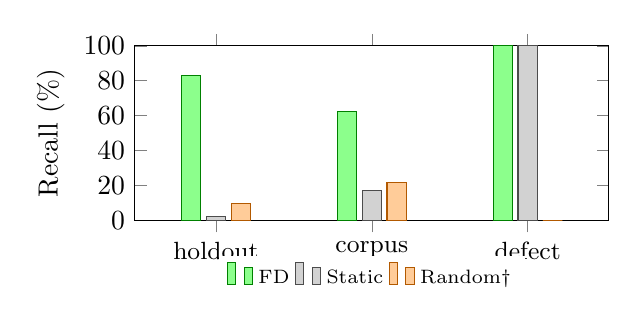
\begin{tikzpicture}
\begin{axis}[
  width=7.6cm, height=3.8cm,
  ybar, bar width=7pt,
  ymin=0, ymax=100,
  ylabel={Recall (\%)},
  symbolic x coords={holdout, corpus, defect},
  xtick=data,
  x tick label style={font=\small},
  legend style={font=\scriptsize, at={(0.5,-0.20)}, anchor=north, legend columns=3, draw=none},
  enlarge x limits=0.26,
  title style={font=\small},
]
\addplot[fill=green!45, draw=green!50!black] coordinates {(holdout,82.9) (corpus,62.5) (defect,100)};
\addplot[fill=gray!35, draw=gray!60!black] coordinates {(holdout,2.4) (corpus,17.2) (defect,100)};
\addplot[fill=orange!40, draw=orange!70!black] coordinates {(holdout,9.8) (corpus,21.9) (defect,0)};
\legend{FD, Static, Random$\dagger$}
\end{axis}
\end{tikzpicture}
\caption{Core recall across three arms on the expanded samples. \textbf{FD} holdout 82.9\%
[67.9, 92.8] / corpus 62.5\% [49.5, 74.3]; \textbf{Static} (rule-only, a \emph{caliber re-binning},
not a re-run) 2.4\% / 17.2\%; \textbf{Random$\dagger$} (instrument-level \emph{proxy}, not the
paper's B3) 9.8\% / 21.9\%. Point estimates only; Clopper--Pearson 95\% CIs are in
Table~\ref{tab:e1}. $n=41/64$ is small---read \emph{direction} first, magnitude second.}
\label{fig:core}
\end{figure}

\paragraph{E1 --- Main experiment: static vs.\ random vs.\ failure-driven (Figure~\ref{fig:core}).}
The three arms on the same samples (Static caliber re-bin; Random$\dagger$ proxy; FD) give holdout
82.9\% [67.9, 92.8] / corpus 62.5\% [49.5, 74.3] for FD, vs.\ Static 2.4\%/17.2\% and Random$\dagger$ 9.8\%/21.9\%;
$\Delta$(static$\to$FD) is $+80.5$pp/$+45.3$pp and $\Delta$(random$\dagger\to$FD) $+73.2$pp/$+40.6$pp (all CIs strictly positive). Full table in Appendix~\ref{tab:e1}.
\textbf{Expanded-sample honesty:} the expansion moved holdout 81.0\%$\to$\textbf{82.9\%} and corpus
54.2\%$\to$\textbf{62.5\%}; both rises are split into \emph{composition} vs \emph{within-layer}
change, \textbf{not} capability gains. The H4 subset check passes for holdout (+4.0pp) but
\textbf{fails for corpus (+33.3pp)} and is registered as a composition shift. FPR is
\textbf{0.0\%} (0/11 controls); the pre-673u 18.2\% (2/11) came from a constant-catch detector bug
(Appendix~\ref{app:incidents}). All four pre-registered $\Delta$ CIs are strictly positive (lowest
bound 28.6pp).

\paragraph{E2 --- Caliber ablation (Table~\ref{tab:e2}, Fig.~\ref{fig:caliber}).} Three arms share
\emph{the same raw catch counts} (holdout 34, corpus 40) and differ only in the denominator: A (main;
drop unknown) gives \textbf{82.9\%/62.5\%}, B (unknown$\to$miss) 81.0\%/54.8\%, C (all samples)
81.0\%/52.6\%. The caliber effect on the external corpus reaches $\mathbf{+9.9}$pp, so a rate without
its caliber is uninterpretable---a reader could pick anywhere in 52.6--62.5\%.

\begin{figure}[t]
\centering
\begin{minipage}[t]{0.48\linewidth}
\centering
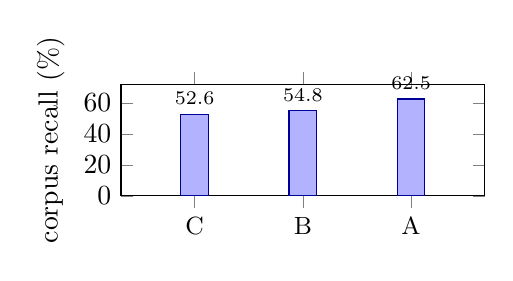
\begin{tikzpicture}
\begin{axis}[
  width=6.2cm, height=3.0cm,
  ybar, bar width=10pt,
  ymin=0, ymax=72,
  ylabel={corpus recall (\%)},
  symbolic x coords={C, B, A},
  xtick=data,
  x tick label style={font=\small},
  nodes near coords, nodes near coords style={font=\scriptsize},
  enlarge x limits=0.34,
]
\addplot[fill=blue!30, draw=blue!60!black] coordinates {(C,52.6) (B,54.8) (A,62.5)};
\end{axis}
\end{tikzpicture}
\caption{Caliber ablation on the external corpus: the \emph{same} 40 catches, three
denominators---C (all samples) 52.6\%, B ($+$unknown) 54.8\%, A (main) 62.5\%: a \textbf{+9.9}pp
swing from the caliber alone (holdout: $+1.9$pp).}
\label{fig:caliber}
\end{minipage}\hfill
\begin{minipage}[t]{0.48\linewidth}
\centering
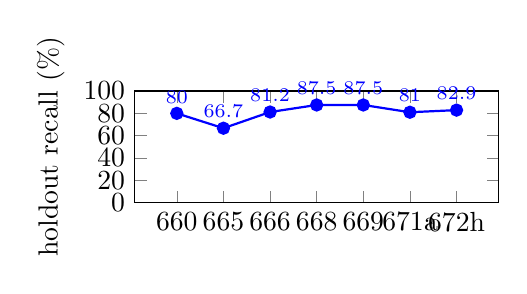
\begin{tikzpicture}
\begin{axis}[
  width=6.2cm, height=3.0cm,
  ymin=0, ymax=100, ylabel={holdout recall (\%)},
  symbolic x coords={660,665,666,668,669,671a,672h}, xtick=data,
  nodes near coords, nodes near coords style={font=\scriptsize},
  enlarge x limits=0.15,
]
\addplot[mark=*, thick, blue] coordinates {(660,80.0) (665,66.7) (666,81.2) (668,87.5) (669,87.5) (671a,81.0) (672h,82.9)};
\end{axis}
\end{tikzpicture}
\caption{Evolution curve. \textbf{80.0$\to$66.7$\to$87.5$\to$81.0$\to$82.9 is not a capability
curve}: 665 is single-flag and 668 dual-flag---detector unchanged; the 666 value (81.2\%) never
landed in any artifact.}
\label{fig:evolution}
\end{minipage}
\end{figure}

\paragraph{E3 --- Evolution curve (cross-batch metrics in Table~\ref{tab:e3}).}
The holdout column is \emph{not the same $X$}: the only same-sample re-measurement is 668 vs.\ 665,
and it changed the \emph{flag}, not the capability.

\paragraph{E4 --- Ablation A5 (\emph{run}): the budget-matched control.}
A0--A4 remain design-only; \textbf{the key contrast A0 $-$ A5} is the core-mechanism falsifier:
\textbf{if the CI of $\Delta(\text{A0}-\text{A5})$ crosses 0, ``failure-driven beats same-budget
random'' does not hold}. It has \textbf{run at full scale} (676f): a real $1137\times8$ matrix,
failure-hits from a disjoint derivation split ($n{=}571$), evaluation on the held-out split
($n{=}566\gg138$). At $k{=}4$ against a 2000-draw random distribution, FD \textbf{54.6\%} vs.\
Random \textbf{30.6\%} ($\Delta{=}\mathbf{+24.0}$pp, CI [+20.5, +27.5],
$p{=}2.3\times10^{-41}$) and vs.\ Static \textbf{24.7\%} ($\Delta{=}\mathbf{+29.9}$pp).
\textbf{The Static contrast is robust; the Random one is not:} excluding the three degenerate
assets, FD-vs-Static \emph{grows} to \textbf{+30.6}pp while FD-vs-Random collapses to \textbf{0.0}pp
($p{=}1.0$)---Random's draw is then the same four. A5 isolates ``do not fund assets that cannot
inform,'' not ``a smarter ranking''; we still do not write ``FD beats Random''. A 676m label
re-check left this endpoint \emph{bit-identical} (Appendix~\ref{app:a5full}).
\textbf{Robustness (677b/677c, Appendix~\ref{app:a5full}).} Clone-family splits leave $\Delta$ at
$+23.0$--$+26.7$pp (leakage is not driving it), but a family-level bootstrap cuts the effective $n$
to $\approx133$--$140$; on the degenerate-free pool the effect survives at $k\le3$ ($+11.31$pp at
$k{=}1$) and the $k{=}4$ zero is a set collision.

\paragraph{E5 --- Statistical tests for the baseline contrasts (Table~\ref{tab:e5}).}
FD and the two opponent arms are paired \emph{on the same samples} (41 / 64 pairs), so we use exact
McNemar on the paired risk difference with Clopper--Pearson intervals. Small-sample warning:
McNemar rests on the extreme $c{=}0$ structure---a few reverse pairs would inflate $p$ quickly.
Holm/Bonferroni over the four pre-registered contrasts leaves all significant
($p_{\max}=1.2\times10^{-7}$); the correction changes no conclusion, but the discipline requires it.
Cohen's $h$ is reported for \emph{sensitivity only}: the design is paired, so the paired $\Delta$
and its interval are our primary effect measures (Appendix~\ref{app:stats}).

\paragraph{E7--E8 --- LLM judge arm and external anchor (both negative).}
An LLM judge (\textbf{GLM-4}) caught \textbf{12/12} errors vs.\ FD's 6/12 on the same subset but
produced \textbf{4/8} false positives on controls (\emph{more sensitive, far less specific}); an
external anchor on the \textbf{C++ Core Guidelines} gives \textbf{44.0\%} over 50 snippets, with
pre-registered \textbf{H2 missing by 0.8pp}. Both are reported without ``correction''
(Appendix~\ref{app:extra}).

\paragraph{E9 --- Cross-regime external stress test (clang-tidy / cppcheck).}
On the \emph{same} 41/64 samples, under the only defensible caliber (StrictA, chosen \emph{after}
results, hence exploratory), FD \textbf{82.9\% (34/41)} beats clang-analyzer \textbf{48.8\% (20/41)}
and cppcheck \textbf{41.5\% (17/41)} on holdout ($p{=}1.2\times10^{-4}$ / $1.5\times10^{-5}$) but only
\emph{ties} cppcheck on corpus (62.5\% vs.\ 54.7\%, $p{=}0.383$)---complementary regimes, a
stress test rather than a ranking (Appendix~\ref{app:clangtidy}).

% =====================================================================
\section{Analysis}
\label{sec:analysis}
% =====================================================================
\textbf{(1) Labels are the largest error source.} A batch reported ``20 holdout samples'' of which only
\textbf{7} were true errors: the same data reads 35\% or 80.0\% by denominator---the \emph{measured
object} was corrected, not the verifier. \textbf{(2) Environment dependence causes silent drops:}
without WSL, 15 samples degrade to \texttt{unknown} and external recall falls
\textbf{35.0\%$\to$10.0\%} \emph{with the guard green}. \textbf{(3) Apparatus drift is systematic:}
three audited instances in which the reported number and the artifact disagreed because code changed
without re-measurement (Appendix~\ref{app:incidents})---a rate can be \emph{hollow} unless a
field-complete recomputation is run. \textbf{(4) Mutation score $\neq$ real defect detection:}
internal core \textbf{96.5\%} (110/114) vs external \textbf{62.5\%} (40/64); mutants correlate with,
but do not equal, real faults~\cite{just2014mutants}.
\textbf{(5) Whether FD gains are real.} FD beats the static and random-proxy arms
($p\le3.0\times10^{-8}$), but that random arm is an \emph{instrument-level proxy}; the real A5
control, significant at $n{=}566$, \emph{survives} on the degenerate-free pool only at $k\le3$
($+7.4$ to $+11.3$pp, the $k{=}4$ zero being a set collision), carries an effective
$n\approx133$--$140$, and is unchanged by clone-family splitting. So ``FD beats same-budget
random'' stays \emph{directional}---about a smaller, better-identified effect (\S\ref{sec:exp}).

% =====================================================================
\section{Threats to Validity}
\label{sec:validity}
% =====================================================================

The nineteen threats and their mitigations/residuals are in Table~\ref{tab:threats}; the
residual-validity matrix in Table~\ref{tab:validity}.

\paragraph{Biggest unresolved threat: unreviewed labels; and the pinning gap.}
All detection rates rest on human-authored labels (41 holdout $+$ 64 corpus) with a single annotator
and \emph{no} IRR---a mislabeled sample moves a rate silently in either direction. We pre-registered
a two-annotator re-label of a random 25\% subsample ($10/41$, $16/64$), original annotator blinded,
$\kappa<0.6$ escalating to a $100\%$ third-party re-review, before any ``verified'' claim.
Historical-state pinning is separately \emph{incomplete}: current-state verdicts are fully
reproducible, historical ones only under an unchanged-ruleset assumption, and the guard does not
re-run detectors (Appendix~\ref{app:pinning}).

\paragraph{Instrument boundary; A5's remaining gaps (all measured).}
Over $1147$ samples \textbf{38.4\%} are blind spots ($13$ of $34$ normalized types exceed $50\%$), so every
rate here speaks about the \emph{visible} region only (Appendix~\ref{app:blindspot}). For A5, power
is closed ($n{=}566$) and \emph{identification} is not (Appendix~\ref{app:threats_quantified}).
\emph{Two measured corrections to that reading.} \textbf{Effective sample size:} the samples are
template clones (474 families), and a family-level cluster bootstrap gives a design effect of
$\approx4.1$--$4.3$---\textbf{effective $n\approx133$--$140$}, not $566$, so all A5 intervals widen
by $1.8$--$2.1\times$ ($\Delta$ on the clone-aware splits: $[+16.6,+30.4]$pp and $[+18.3,+33.4]$pp,
both excluding 0). \textbf{Degenerate assets:} $\approx$\,$+12$pp of the full-pool
$\Delta{=}+24.0$pp is degenerate-asset avoidance, leaving an isolated selection effect of
$\approx$\,$+7$--$12$pp---that smaller number is the mechanism-level estimate
(Appendix~\ref{app:a5full}).

\paragraph{Three scope restrictions on reading our numbers.}
\textbf{(i)} the blind-spot ratio is an \emph{instrument-boundary} statistic---\textbf{38.4\%} is
measured \emph{on our 1147-sample corpus with our 8-asset instrument} and is expected to move when
either changes; \textbf{(ii)} the $74$ \texttt{planted=false} samples are single-file
\emph{reconstructions} of real CVEs/issues, not production code (Appendix~\ref{app:datasheet});
\textbf{(iii)} a \texttt{pass} concerns \emph{acquired evidence within a boundary}, not semantic
correctness (\S\ref{sec:terminology}).

% =====================================================================
\section{Claim Boundary}
\label{sec:claim}
% =====================================================================

The falsifiable claim boundary---every claim asserted, refused, or left unknown---is enumerated in
Table~\ref{tab:claim} (Appendix~\ref{app:tables}). We state the most important boundary first,
because it bounds every other entry:

\textbf{C0. Queyi does not verify semantic truth; it evolves an evidence-acquisition apparatus.}
A \texttt{pass} means \emph{no acquired evidence contradicts the assertion within the current
capability boundary}---not that it is true, correct, or free of defects outside that boundary. On
our corpus \textbf{38.4\%} of samples are invisible to our 8-asset instrument, so \emph{every} rate
here concerns the visible region only (\S\ref{sec:terminology}, Appendix~\ref{app:blindspot}).
All remaining claims---supported, refused, unknown---are in Table~\ref{tab:claim}, and the
e-process is \emph{exploratory} and supports none of them (Appendix~\ref{app:eprocess}).

% =====================================================================
\section{Conclusion}
\label{sec:conclusion}
% =====================================================================
LLMs drive the \emph{generation} cost of technical knowledge to near zero, but the
\emph{verification} cost does not fall. It cannot be solved by model-judging-model (shared failure
domain) or AI-text detection (wrong question), but by binding
\emph{verdict--evidence--recomputation} into a chain an external party can interrupt---which Queyi
realizes as four auditable mechanisms: four-state verdicts (\texttt{unknown} first class), a
forced provenance/semantic-scope split, a kernel-independent meta-state reconciler, and a
failure-driven loop.

We also made our own failures part of the method: 66.7\%$\to$87.5\% is a caliber change (the old
value must be voided), and \textbf{81.0\%$\to$82.9\% and 54.2\%$\to$62.5\% are expanded-sample
re-estimates, not capability gains}. The recurring lesson is that \textbf{apparatus state is not
self-announcing}: a rate can be reported while no artifact contains it, and no check we own detects
this today (Appendix~\ref{app:incidents}). A third-party audit rates overall credibility
\textbf{6/10}: infrastructure trustworthy, \emph{numbers fragile}.

\textbf{Evidence boundary.} The evidence \emph{supports} external measurability and the advantage over
the static re-binning and random-proxy arms ($\Delta$ lower bound $\ge$28.6pp, exact McNemar
$p\le3.0\times10^{-8}$); it does \emph{not} support superiority over a \emph{real} static detector or a
true B3, other languages, ``exact magnitudes'' ($n{=}41/64$), or ``FD beats same-budget
random''---A5 runs at $n{=}566$: the \emph{Static} contrast is robust (\textbf{+29.9}pp;
\textbf{+30.6}pp in the parallel analysis), while the \emph{Random} contrast is \textbf{+11.3}pp at
$k{=}1$ on the degenerate-free pool and \textbf{0.0}pp at $k{=}4$ (a set collision, not a mechanism
failure). \textbf{Our central empirical result is therefore directional:} failure-driven selection
is worth $\approx$\,$+7$--$12$pp on usable assets, unchanged under clone-family splitting, with an
\emph{effective} $n\approx133$--$140$---evidence \emph{for the mechanism}, not a confirmatory
demonstration.
\textbf{Qualifiers:} the $\Delta$ concerns \emph{having runtime evidence}, not failure-driven
selection; E9 is a stress test; labels have only AI self-agreement ($\kappa{=}0.77$; T17); and
\textbf{38.4\%} of $1147$ samples are blind spots \emph{on our corpus with our 8-asset instrument},
so no rate here speaks about deadlock or interrupt safety (\S\ref{app:blindspot}). \textbf{Next:}
A0--A4 and multi-round verdicts (the non-degenerate pool has now run; Appendix~\ref{app:future}).

\paragraph{What this changes about how evaluation should be designed.}
The transferable content is not the 67 rules and not the 82.9\%---it is three design obligations
cheap to meet and expensive to violate: \textbf{(1)} \emph{report the instrument boundary with every
rate} (one sample$\times$asset matrix is all it costs); \textbf{(2)} \emph{bind every rate to a
declared caliber and recompute it from artifacts} (caliber alone moved our corpus rate by
\textbf{9.9pp} with the raw catches unchanged); \textbf{(3)} \emph{make the apparatus's own failures
the only legal input to its evolution, under external interrupt}---otherwise evolution is
indistinguishable from Goodhartization, whereas a
\texttt{failure}$\to$\texttt{rule}$\to$\texttt{re-test} chain makes ``the instrument got wider''
externally checkable. None of the three is domain-specific.

\clearpage
\label{page:endmain}% records the page where the main text ends (for the 9-page check)
\bibliographystyle{plainnat}
\bibliography{queyi_refs}

% =====================================================================
\newpage
\appendix

\section{LLM Arm and External Anchor (details)}
\label{app:extra}
\paragraph{E7 --- LLM judge arm (result \emph{opposite} to expectation, registered as such).}
A paired arm gave the same samples (6 catch $+$ 6 miss $+$ 8 control) to \textbf{GLM-4}
(temperature 0.01, prompt v1). It caught \textbf{12/12} errors vs.\ FD's 6/12 on the same subset, but
produced \textbf{4/8 false positives} (\textbf{50\%}) on controls (item-wise agreement 0.50; exact
McNemar favours the LLM, $b{=}0$, $c{=}6$, $p{=}0.031$). \textbf{All four pre-registered hypotheses
failed}: the LLM is \emph{more sensitive but far less specific}. Two caveats: some samples carry
\texttt{answer\_leak\_risk} (fixture comments may hint the answer), so ``judging'' cannot be fully
separated from ``reading the answer''; and it is a single model on a single prompt. This is the
empirical case for T15---an LLM may \emph{propose}, but its output never becomes a verdict.

\paragraph{E8 --- External anchor (C++ Core Guidelines; H2 misses by 0.8pp).}
We scanned the official \textbf{C++ Core Guidelines} (\texttt{isocpp/CppCoreGuidelines}, sha256
\texttt{27b53e7d\ldots}), taking one compilable snippet per rule in document order (87 rules). The two
subsets are reported \emph{separately} because their targets differ: \textbf{A} verbatim guideline
snippets (35 measurable, \textbf{28.6\%} [14.6, 46.3]) and \textbf{B} reconstructed UB fragments
(15, \textbf{80.0\%}); total \textbf{44.0\%} over 50. A is low because most guideline text is
stylistic advice rather than an executable error---``no detection'' there is \emph{expected}, not a
miss; B is our own reconstruction (\texttt{verified\_source=false}) and is therefore an \emph{upper
bound}. Pre-registered verdicts: H1/H3 hold, \textbf{H2 misses by 0.8pp} and is registered as
\emph{not} passed. A harness (\texttt{prelude\_v1}) was added post-registration because raw
compilability was 11/60; the deviation is logged and does not change hypotheses or thresholds.

\section{Threat, Validity and Evolution Tables}
\label{app:tables}
Layer read at 672h (k/n per layer; layers are never merged): corpus sanitizer
\textbf{85.3\%} (29/34), compiler-warn \textbf{50.0\%} (9/18), cross-compile \textbf{16.7\%}
(2/12)---three further layers lack local detectors and therefore claim \emph{no} rate; holdout
sanitizer \textbf{84.6\%} (33/39). These denominators are recomputed from the landed reveal
artifacts and are the source of the abstract's layered read.

\begin{table}[t]
\caption{E4. Ablation groups A0--A5. Each row writes its hypothesis \emph{before} results.}
\label{tab:e4}
\centering
\footnotesize
\begin{tabular}{@{}clp{2.9cm}p{3.1cm}p{4.7cm}@{}}
\toprule
ID & Remove/change & Hypothesis & Primary metric & Result \\
\midrule
A0 & Full system (baseline) & --- & detection rate & \texttt{\{\{TODO\_ablation\_A0\}\}} \\
A1 & $-$failure-derived rules (post-657 ruleset) & H: detection drops & $\Delta$ detection vs.\ A0 & \texttt{\{\{TODO\_ablation\_A1\}\}} \\
A2 & $-$holdout isolation (blind$\to$dev) & H: overfitting (dev$\uparrow$, blind flat) & dev vs.\ blind recall & \texttt{\{\{TODO\_ablation\_A2\}\}} \\
A3 & $-$provenance (boundary-triple check) & H: false-pass rate rises & false-pass rate & \texttt{\{\{TODO\_ablation\_A3\}\}} \\
A4 & $-$mutation (L1 self-justification) & H: internal strength drops & mutation kill (internal) & \texttt{\{\{TODO\_ablation\_A4\}\}} \\
A5 & random-budget control & H: below A0 & $\Delta$ detection vs.\ A0 & \textbf{run at full scale (676f)}: $n{=}566$ eval; vs Random \textbf{+24.0}pp [+20.5, +27.5] ($p{=}2.3{\times}10^{-41}$), vs Static \textbf{+29.9}pp ($p{=}1.9{\times}10^{-31}$); Static contrast survives the parallel analysis (\textbf{+30.6}pp), Random contrast collapses to \textbf{0.0}pp $\Rightarrow$ \texttt{uninterpretable} \\
\bottomrule
\end{tabular}
\end{table}
\begin{table}[h]
\caption{E5. Paired contrasts on the same samples. $b$ = FD catch \& opponent miss;
$c$ = opponent catch \& FD miss. All four contrasts have $c=0$ (the opponent's catches are a
subset of FD's), so the difference comes entirely from samples only FD catches.}
\label{tab:e5}
\centering
\footnotesize
\begin{tabular}{@{}llrll@{}}
\toprule
Contrast & Set & $(b, c)$ & exact McNemar $p$ & Cohen's $h$ \\
\midrule
FD vs.\ Static & holdout ($n{=}41$) & (33, 0) & $2.3\times10^{-10}$ & \textbf{1.98} (large) \\
FD vs.\ Static & corpus ($n{=}64$) & (29, 0) & $3.7\times10^{-9}$ & \textbf{0.97} (large) \\
FD vs.\ Random$\dagger$ & holdout ($n{=}41$) & (30, 0) & $1.9\times10^{-9}$ & \textbf{1.65} (large) \\
FD vs.\ Random$\dagger$ & corpus ($n{=}64$) & (26, 0) & $3.0\times10^{-8}$ & \textbf{0.85} (large) \\
\bottomrule
\end{tabular}
\end{table}

\begin{table}[h]
\caption{Baselines and their alignment conditions (moved from main text; referenced in \S\ref{sec:baseline}).}
\label{tab:baseline}
\centering
\footnotesize
\begin{tabular}{@{}lp{5.2cm}p{6.4cm}@{}}
\toprule
Baseline & Definition & Alignment \\
\midrule
B1 static gate & static rules only (no runtime evidence) & same corpus, same verdict granularity \\
B2 static $+$ mutation & static rules $+$ mutation testing & same as above $+$ same mutation budget \\
\textbf{B3 budget-matched random} & random evidence acquisition under \emph{equal budget} & same budget (time/calls), same corpus, same flags \\
\bottomrule
\end{tabular}
\end{table}

\begin{table}[h]
\caption{Four-state verdict (moved from main text; referenced in \S\ref{sec:method}).}
\label{tab:verdict}
\centering
\footnotesize
\begin{tabular}{@{}lll@{}}
\toprule
State & Meaning & Action \\
\midrule
\texttt{pass} & evidence supports the assertion; boundary triple complete & may enter the teaching ledger \\
\texttt{fail} & evidence contradicts the assertion & counterexample to the teaching set \\
\texttt{unknown} & insufficient evidence or detector unavailable & never recorded as pass/miss; reported separately \\
\texttt{contradict} & two pieces of evidence conflict (e.g.\ cross-compiler) & escalated to human review; no machine pick \\
\bottomrule
\end{tabular}
\end{table}

\begin{table}[h]
\caption{E2. Caliber ablation (same raw counts, different denominator). The 669d table
(87.5/82.4/82.4 and 43.8/37.8/35.0) is \emph{retired}: its denominators are the pre-expansion
16/17/40. Moved from main text; referenced in \S\ref{sec:exp}.}
\label{tab:e2}
\centering
\footnotesize
\begin{tabular}{@{}lp{3.6cm}p{3.6cm}p{3.6cm}@{}}
\toprule
Arm & Caliber & holdout (CP 95\%) & external (CP 95\%) \\
\midrule
\textbf{A (main; drop unknown)} & denominator $=$ catch$+$miss & \textbf{82.9\% (34/41) [67.9, 92.8]} & \textbf{62.5\% (40/64) [49.5, 74.3]} \\
B (unknown $\to$ miss) & denominator incl.\ detector-unknown & 81.0\% (34/42) [65.9, 91.4] & 54.8\% (40/73) [42.7, 66.5] \\
C (unknown $+$ not\_error) & denominator $=$ all samples & 81.0\% (34/42) [65.9, 91.4] & 52.6\% (40/76) [40.8, 64.2] \\
\midrule
$\Delta$(A$-$C) & & $+1.9$pp & $\mathbf{+9.9}$pp \\
\bottomrule
\end{tabular}
\end{table}

\begin{table}[h]
\caption{E1. Three arms on the same samples. Static is a caliber re-binning; Random$\dagger$ is a
proxy (the real B3 needs the split-repo \texttt{select\_assets}). Moved from main text; referenced in \S\ref{sec:exp}.}
\label{tab:e1}
\centering
\footnotesize
\begin{tabular}{@{}lp{2.7cm}p{2.4cm}p{1.7cm}p{1.5cm}@{}}
\toprule
System & Blind holdout (CP 95\%) & Corpus meas.\ (CP 95\%) & Defect & Control FPR \\
\midrule
Static (caliber re-bin) & 2.4\% (1/41) [0.1, 12.9] & 17.2\% (11/64) [8.9, 28.7] & 100\% (6/6) & --- \\
Random$\dagger$ (proxy) & 9.8\% (4/41) [2.7, 23.1] & 21.9\% (14/64) [12.5, 34.0] & N/A & --- \\
\textbf{FD (failure-driven)} & \textbf{82.9\% (34/41) [67.9, 92.8]} & \textbf{62.5\% (40/64) [49.5, 74.3]} & 100\% (6/6) & 0.0\% (0/11) [0.0, 28.5] \\
$\Delta$(static$\to$FD) & \textbf{+80.5pp} [68.4, 92.6] & \textbf{+45.3pp} [33.1, 57.5] & 0 & --- \\
$\Delta$(random$\dagger\to$FD) & \textbf{+73.2pp} [59.6, 86.7] & \textbf{+40.6pp} [28.6, 52.7] & N/A & --- \\
\bottomrule
\end{tabular}
\end{table}

\section{Rule Pinning and e-Process (details)}
\label{app:pinning}
\textbf{Rule-version pinning (design principle; manifest-level today).} Rules inevitably evolve, so
a ledger that records only verdicts cannot let a third party recompute a one-year-old decision: the
ruleset of the day must be pinned. We snapshot the ruleset and hash the canonicalised manifest into
\texttt{rules\_manifest\_sha256}, archived append-only, with each ledger event double-referencing
that hash and the evidence-toolchain snapshot. \textbf{Current state (measured):} the manifest
exists (\texttt{rules\_sha256}, version 1.0.0, 67 rules), but the \textbf{452 ledger events do not
yet carry the field}---backfilling is registered as future work, so today a historical recomputation
must \emph{assume} the ruleset was unchanged.

\textbf{e-process (moved).} The sequential-testing layer is described in full in
Appendix~\ref{app:eprocess}; it is \textbf{exploratory} and supports no confirmatory claim in this
paper.

\section{E-Process (exploratory)}
\label{app:eprocess}
\textbf{EXPLORATORY --- not pre-registered, not used for confirmatory claims.} $\mu_0$ is not
frozen, the alternative grid and the mixing prior are not frozen, the implementation is not in CI,
and no claim in this paper depends on an e-value. We publish it because (i) it is the natural
anytime-valid companion to an append-only ledger and (ii) we want the fact that it is
\emph{not} ready to be on the record rather than discovered by a reader.

\textbf{Why an e-process at all.} The ledger accumulates items one
at a time, yet rates are reported at snapshots---that is \emph{peeking}. We treat each event as a
binary observation, mix likelihood ratios over a grid of alternatives, and obtain an \emph{e-process}
(a non-negative supermartingale with expectation 1 under $H_0$); the cumulative e-value is
\emph{multiplied} by one factor per new item, and we reject when $\sup_t e_t \ge 1/\alpha$ (i.e.\ 20
at $\alpha{=}0.05$). Ville's inequality guarantees that peeking at \emph{any} time keeps the
type-I error at $\alpha$, so expansion needs no re-calibration, and the e-values \emph{multiply
across batches}---isomorphic to an append-only ledger. Measured, the FD contrasts reach e-values of
$2.5\times10^8$ / $1.8\times10^7$ (static) and $3.5\times10^7$ / $2.5\times10^6$ (random), far
above the threshold of 20---\emph{but these are exploratory numbers}: because $\mu_0$ and the
alternative grid are not pre-registered, a reader who chooses them differently gets different
e-values, and the margin above 20 is therefore \emph{not} a measure of evidence strength.
\textbf{Honest boundaries:} the anytime-valid price is a threshold of
$\approx$20 versus $\approx$3.14 for a single fixed-sample test ($\approx$6.4$\times$ in
likelihood-ratio terms), so the e-value here is a \emph{safety belt for expansion and a cross-batch
evidence combiner}, not the primary test; and the implementation is a preliminary not yet in CI.
\textbf{Difference from CELEUS}~\cite{zhou2026celeus}: CELEUS uses e-processes to \emph{save
samples} in LLM evaluation; we use them for anytime-valid, third-party-recomputable decisions over a
\emph{knowledge-assertion} ledger. We do \emph{not} claim to be first.


\begin{table}[t]
\caption{Positioning: six works $\times$ five dimensions. Benchmark evolution evolves the
\emph{items}; MiniCheck evolves the \emph{judge} (a trained fact-checking model); Queyi evolves
the \emph{verifier's evidence-acquisition capability} while requiring every step of that
evolution to be externally measurable.}
\label{tab:positioning}
\centering
\footnotesize
\begin{tabular}{@{}p{2.5cm}p{2.2cm}p{2.6cm}p{2.2cm}p{2.1cm}p{2.0cm}@{}}
\toprule
Work & Object evolved & Strategy & Auditable & Failure-driven & 4-state \\
\midrule
Benchmark Self-Evolving~\cite{wang2024benchmarkevolving} & items / samples & model-feedback rewriting & partial (generation logs) & no (pass/difficulty signal) & no \\
ArenaBencher~\cite{liu2025arenabencher} & items (adversarial) & opponent-model games & partial & no (win-rate signal) & no \\
LiveBench~\cite{white2024livebench} & items (periodic refresh) & human $+$ model updates & partial (item dates) & no (temporal rotation) & no \\
SWE-bench Verified~\cite{jimenez2024swebench,liang2025illusion} & items (human filtering) & manual subset curation & high (human review) & no (static set) & no \\
MiniCheck~\cite{tang2024minicheck} & the judge (fact-check weights) & distillation training & no (trusts the model) & no (training objective) & no \\
\textbf{Queyi (ours)} & \textbf{verifier capability $\mathcal{C}$} & \textbf{failure-driven: \texttt{miss}/\texttt{unknown} $\to$ new detectors/rules} & \textbf{Merkle $+$ 452-event ledger $+$ per-sample detail} & \textbf{yes (only legal input)} & \textbf{yes (\texttt{unknown}/\texttt{contradict} first-class)} \\
\bottomrule
\end{tabular}
\end{table}
\begin{table}[t]
\caption{What the current evidence does and does not support.}
\label{tab:claim}
\centering
\small
\begin{tabular}{@{}p{1.3cm}p{5.4cm}p{7.0cm}@{}}
\toprule
 & Claim & Evidence \\
\midrule
\cmark\ supported & High recall on \emph{seen} error types & holdout \textbf{82.9\%} (34/41) [67.9, 92.8]; corpus measurable \textbf{62.5\%} (40/64) [49.5, 74.3] (post-672h) \\
\cmark\ supported & Gates catch \emph{known} defects (change a number, go red) & range self-check 5/5 red; gate \texttt{overall=PASS} \\
\cmark\ supported & Provenance chain fully auditable & 5 Merkle roots consistent; 452-event ledger unchanged; provenance triple landed \\
\cmark\ supported & Caliber declarable and recomputable & three-arm caliber ablation; every rate carries a denominator \\
\cmark\ supported & On the same samples FD beats the static re-binning and random$\dagger$ proxy arms & exact McNemar $p\le3.0\times10^{-8}$; Cohen's $h\ge0.85$; $\Delta$ lower bound $\ge$28.6pp (\S\ref{sec:exp}) \\
\cmark\ supported & Verifier semantic coverage and evolution rate are measurable & Verifier Coverage 31/42 = 73.8\% (descriptive census over our fixed 42-card claim set; no CI---see \S\ref{sec:exp}); EE 1.9pp/rule (descriptive; \S\ref{sec:method}) \\
\cmark\ supported & On the \emph{visible} region, FD beats a budget-matched static arm at scale & A5: +29.9pp ($p{=}1.9\times10^{-31}$), +30.6pp in the parallel analysis ($n{=}566$); unchanged under clone-family splitting (677b); effective $n\approx133$--$140$ \\
\cmark\ supported & A detector's capability boundary can be mapped and published & 1147-sample $\times$ 8-asset matrix \emph{on our corpus with our 8-asset instrument}: blind-spot ratio 38.4\%; 18/70 types $>50\%$ blind; union of 6 assets 61.6\% vs best single 35.6\% (\S\ref{app:blindspot}). \emph{Instrument-boundary statistic, not a property of C++ defect detection} \\
\midrule
$\times$ not supported & Generalization to \emph{unseen} error types & all samples same-source; scope backfill 0/26 \\
$\times$ not supported & Absolute ``detection rate $X$\%'' & $n{=}41/64$, CI half-width $\approx$12pp; $\pm$5pp needs $n{=}236/378$ \\
$\times$ not supported & Better than a \emph{real} static detector / true B3, or ``FD beats same-budget random'' & static arm is a caliber re-binning; random$\dagger$ is a proxy; real interfaces BLOCKED; \textbf{A5 at full scale ($n{=}566$) is significant vs Static and robust in the parallel analysis (+30.6pp)}; vs Random it is \textbf{+11.31pp at $k{=}1$ on the degenerate-free pool} ($p{=}6.0\times10^{-8}$; 677c) and 0.0pp at $k{=}4$ (set collision $1/\binom54$); clone-aware splits leave both unchanged (677b) and the family-level cluster bootstrap gives effective $n\approx133$--$140$ $\Rightarrow$ \emph{direction-only} on a smaller selection effect ($\approx$\,$+7$--$12$pp) \\
$\times$ not supported & ``$F_1{=}1.0$ is calibrated'' & criterion and truth are same-source $\Rightarrow$ upper bound \\
$\times$ not supported & Mutation score as detection rate & core 96.5\% $\neq$ defect-detection rate~\cite{just2014mutants} \\
$\times$ not supported & Evolution trend & only a single same-sample re-measurement \\
\midrule
\multicolumn{3}{@{}p{13.7cm}@{}}{\textbf{Not reproducible (fail when the environment changes):} holdout/external recall depend on \textbf{WSL + g++ + \texttt{setarch}} (silent drop 35.0\%$\to$10.0\% without WSL; 669d-era caliber); TSan results are intermittently unavailable under WSL high-entropy ASLR; the OTS anchor is a zero-attestation placeholder, so ``anchored on-chain'' does \emph{not} hold.} \\
\bottomrule
\end{tabular}
\end{table}

The three tables below are moved here to keep the main text within the 9-page limit; their labels are unchanged, so all cross-references still resolve.

\begin{table}[t]
\caption{Threats, mitigations and residual risks.}
\label{tab:threats}
\centering
\small
\begin{tabular}{@{}p{0.5cm}p{4.6cm}p{4.2cm}p{4.6cm}@{}}
\toprule
\# & Threat & Mitigation & Residual \\
\midrule
T1 & Self-justification (toolchain proves itself) & kernel-independent reconciler (\S\ref{sec:reconciler}) & reconciler still needs human review; \texttt{--check} $\neq$ independent implementation \\
T2 & Self-made distribution bias & blind holdout + external corpus (D2/D3) & small external sample \\
T3 & holdout leakage & irreversible reveal; holdout dir not scanned & 10 appended samples have no blinding \\
T4 & developer-knowledge bias & independent generation (A/B/C) & same-process context; not truly independent \\
T5 & caliber drift & meta-state reconciliation & covers registered fields only \\
T6 & semantic-scope misuse & forced provenance/scope split (\S\ref{sec:prov}) & scope completeness 0/26 \\
T7 & metric confusion (mutation $\to$ detection) & metric layering; mutation is self-justification only & external readers may still misread \\
T8 & selection bias (budget) & budget-matched random baseline (\S\ref{sec:baseline}); three arms \textbf{run} & random arm is an \emph{instrument-level proxy} (true B3 not rerun at 672h) \\
T9 & overfitting historical defects & blind D2 + external D3 & appended samples unblinded \\
T10 & reproducibility crisis & Merkle roots + version capture + time anchor & OTS is a placeholder; WSL dependency undeclared \\
T11 & authority manipulation & 452-event ledger, zero-change red line & discipline, not cryptographic enforcement \\
T12 & unclear AI authorship & AI-use registry & contribution split remains a convention \\
T13 & \textbf{peeking / selective stopping}: the ledger accumulates while rates are reported at snapshots & frozen statistical plan; \textbf{e-process / confidence sequence} as a pre-committed expansion protocol (\S\ref{sec:method}) & nothing forces $\mu_0$ to be fixed in advance $\Rightarrow$ pre-registration required \\
T14 & \textbf{four-layer contamination}: literal / near-duplicate / semantic / procedural---can be ``inflated but reproducible'' & paired counterfactual probes (rename identifiers, change compiler/order); unsealing event log; four-layer de-duplication & passive cleaning is unreliable; probes need human reading \\
T15 & \textbf{untrusted LLM channel}: prompt injection / adversarial input (CVE-2025-59145 CamoLeak, CVSS 9.6; indirect-injection ASR 24--52.77\%) & prompt-level spotlighting/datamarking; structural schema check; \textbf{architectural: LLM output never becomes a verdict, ML detection warns but never blocks} & touch-point registry not done; the LLM arm's false-positive rate is 50\% (\S\ref{sec:exp}) \\
T16 & \textbf{small-sample poisoning}: \textbf{250} malicious samples (0.00016\% of tokens) reliably plant a backdoor---the decisive variable is the \emph{absolute count}; our $n{=}41/64$ lies in that range & canary cards; paired counterfactual probes; the reconciler uses a \emph{different} dependency set; candidates run sandboxed as untrusted code & no safety margin; passive cleaning unreliable (3\% poisoning moves the error rate 3\%$\to$24\%) \\
\bottomrule
\end{tabular}
\end{table}
\begin{table}[t]
\caption{Five validity layers: threat / mitigation / residual.}
\label{tab:validity}
\centering
\small
\begin{tabular}{@{}p{1.8cm}p{4.4cm}p{4.0cm}p{3.6cm}@{}}
\toprule
Layer & Threat & Mitigation & Residual \\
\midrule
Construct & \texttt{catch} $\neq$ truth; A/B/C split by detector availability not difficulty; mutation score not a detection proxy~\cite{just2014mutants}; \textbf{static arm is a caliber re-binning, not a re-run; random$\dagger$ is an instrument-level proxy, not B3} & caliber/denominator/opt\_levels/env stored with artifacts; dual-flag; three-state separation; proxy arms marked $\dagger$ and excluded from conclusions & cross-environment reproduction unverified (upgraded from ``residual'' to ``observed failure'': score drops without WSL); no independent label review; ``with/without runtime evidence'' vs.\ ``failure-driven'' not yet separated (needs ablation) \\
Internal & meta-Goodhart; budget selection bias; code changed without rerun & caliber three-step discipline; range self-check (5/5 turn red); budget-matched random control & guard does not rerun the detector, so the 666 incident can recur; A5 run but holds only as pool composition (\texttt{uninterpretable}); A0--A4 design frozen \\
External & small $n$ (holdout 21 / corpus 48 measurable); \textbf{expanded samples merged after reveal (no blind state: 10 holdout $+$ 20 corpus)}; same-source clustering; scope 0/26; single domain (C++) & layered reporting; two sample sets explicitly incomparable; unblinded samples explicitly flagged & static re-bin $+$ random$\dagger$ proxy \emph{run}; \textbf{real B3 BLOCKED}; only A5 run; reconciler is still our own; 0 third-party reproductions \\
Statistical & \textbf{small $n$ (41/64)} $\Rightarrow$ still-wide CIs; McNemar rests on the extreme $c{=}0$ structure; \textbf{control FPR 0.0\% (0/11)}; multiple comparisons; Wald invalid at small $n$; clustering; $p$ without effect size & frozen plan; CP primary, Wilson sensitivity; Fisher/Boschloo $+$ exact McNemar \emph{tool-implemented}; BH/Holm; difference $+$ CI $+$ effect size $+$ e-value required (the e-process is \emph{exploratory} and supports no confirmatory claim; Appendix~\ref{app:eprocess}) & $\pm$5pp needs $n{=}236/378$; $\pm$10pp needs $61/97$; $\Delta{=}15$pp needs $n\approx103$--173 (paired)---\textbf{A5 now has $n{=}566$ and clears this}, so power is no longer binding for A5, but the holdout/corpus headline ($n{=}41/64$) still has $\approx$12pp half-widths; magnitude not readable as exact; IRR not done \\
Temporal & OTS anchor expired~\cite{opentimestamps}; sample aging; environment drift (TSan intermittently fails under WSL high-entropy ASLR) & Merkle roots $+$ hash chain; versions captured with evidence & OTS not really anchored; re-pinning invalidates the anchor; WSL hard dependency undeclared \\
\bottomrule
\end{tabular}
\end{table}
\begin{table}[t]
\caption{E3. Cross-batch key metrics. \textbf{Un-pinned rows:} the 656 mutation cell (\,62.5\%, 30/48)
has \emph{no surviving artifact}---the current reports recompute to 110/114 and 130/159---and the 665
cell (66.7\%) comes from the retired single-flag (\texttt{-O1}) caliber, so neither may be read as a
reproducible result; they are kept only as a record of what was reported at the time.}
\label{tab:e3}
\centering
\small
\begin{tabular}{@{}llp{3.0cm}lp{3.0cm}@{}}
\toprule
Batch & New capability & holdout (true/caliber) & mutation core & Nature \\
\midrule
656 & core PBT/mutation & --- & \textbf{62.5\%} (30/48) & mutants out of range \\
660 & trace layer & true 7, \textbf{80.0\%} (small den.) & --- & label over-claim \\
665 & expand 20$\to$30 & true 17, \textbf{66.7\%} (single flag) & --- & denominator changed \\
666 & claimed dual & \textit{81.2\% never landed} & --- & code changed, no rerun \\
668 & dual-flag rerun & \textbf{87.5\%} (14/16) & --- & \textbf{caliber change} \\
669 & caliber ablation $+$ CI & 87.5\% [61.7, 98.4] & \textbf{96.5\%} (110/114) & mutation still internal \\
671a & expansion $+$ corpus dual-flag & \textbf{81.0\%} (17/21) [58.1, 94.6] (10 unblinded merged) & --- & \textbf{expanded re-estimate} \\
672h & re-expansion (21$\to$41 / 48$\to$64) & \textbf{82.9\%} (34/41) [67.9, 92.8] (20 unblinded merged) & --- & \textbf{expanded re-estimate (H4 corpus shift registered)} \\
\bottomrule
\end{tabular}
\end{table}

\section{Rule Manifest (67 rules)}
\label{app:rules}
The rule engine computes \texttt{len(RULES)}$=$\textbf{67}. By severity: \textbf{block 44 / warn 16
/ advice 7} (total 67). By kind: fact 61 / pedagogy 5 / meta 1. Fields:
\texttt{id, title, severity, kind, quadrant, scope, automated, basis, fix\_hint, check}.
\emph{Correction note:} an earlier draft wrote ``67 (block 0 / warn 176 / advice 55)''; recomputation
gives \textbf{44/16/7} (sum 67), and the old triple cannot be reproduced from the rule table. The
full 67-row list is generated by the command in Appendix~\ref{app:repro} and shipped with the
supplementary material.

\section{Formal Definitions and Gate Tiers (moved from main text)}
\label{app:formal}
This appendix holds the formal statement of \S\ref{sec:method} that was moved out of the main text
to stay within the page limit. Nothing here is new relative to v1.1.

\paragraph{Formal definitions (backing the three contributions).}
\emph{Verifier state} $\mathcal{C}_t$: the set of available evidence-acquisition means (detectors
$\times$ compilers $\times$ flags $\times$ platforms) at time $t$; its discrete form is the
67-rule set. \emph{Failure set} $F_t = \{x : v_t(x) \in \{\texttt{miss}, \texttt{unknown}\}\}$;
\texttt{miss} points directly at a capability gap, while \texttt{unknown} first needs attribution
(measurement-configuration error vs.\ capability gap). \emph{Evolution operator}
$\mathcal{C}_{t+1} = E(\mathcal{C}_t, F_t)$ with three checkable properties:
\emph{monotonicity} ($\mathrm{cov}(\mathcal{C}_{t+1}) \supseteq \mathrm{cov}(\mathcal{C}_t)$---
evolution never removes capability), \emph{minimality} (every application of $E$ must be triggered
by a \emph{registered} failure; no rule inflation without failure evidence), and
\emph{auditability} (each application leaves the triple (registered failure $f$, new rule $r$,
re-test record)). \emph{Information structure of the four states}: each verdict is a Belnap state
$(\mathrm{support},\mathrm{refutation})$ over registered evidence---\texttt{pass}$=(1,0)$,
\texttt{fail}$=(0,1)$, \texttt{unknown}$=(0,0)$, \texttt{contradict}$=(1,1)$---\emph{while
detector availability} is carried as \emph{separate metadata} per item, not as part of the Belnap
state. Merging \texttt{unknown} into \texttt{miss} or \texttt{pass} pollutes the denominator or
manufactures false confidence; the primary estimand therefore conditions on measurable samples
(denominator $=$ catch $+$ miss). \emph{Auditability conditions}:
origin traceability ($\forall v\, \exists (e,r): v = R_r(e)$), state reproducibility (a third party
rebuilds verdict-time inputs from on-disk artifacts), and tamper detectability (any change to a
controlled directory moves the Merkle root; the ledger is append-only)---jointly necessary, and
jointly met \emph{for the current state} only: ledger events do not yet carry a ruleset hash, so
historical replay assumes the ruleset was unchanged.

\paragraph{Evolution operator: executable form (677c).}
$E$ is instantiated as a one-step selector over candidate assets,
$\mathrm{score}(a_j \mid F_t,\mathcal{C}_t) = w_1\,\text{failure\_coverage}
+ w_2\,\text{novel\_coverage} - w_3\,\text{cost} - w_4\,\text{redundancy}$, with
$a^\ast = \arg\max_j \mathrm{score}$ (ties by ascending id) and
$\mathcal{C}_{t+1} = \mathcal{C}_t \cup \{a^\ast\}$, iterated to $k$ assets; the default weights
$(0.3,0.4,0.1,0.2)$ are \emph{not} learned. Two disclosures. (i) \textbf{The literal specification
collapses:} $F_t$ is by definition the set $\mathcal{C}_t$ misses, so ``novel coverage'' reduces to
failure coverage ($\text{novel}\equiv\text{failure}$), and the operator differs from the greedy
residual-coverage baseline only through the cost/redundancy penalties; we report an
\emph{exploratory} unique-novel variant rather than silently redefining the reference set.
(ii) \textbf{The current FD arm is the frequency-only special case} (global derivation fail-hit
ranking, $w_1{=}1$), so 677c's observation that frequency $\equiv$ FD is a property of the
implementation, not a statement about the mechanism. Ablation over 3 pools $\times$ $k$ tiers: the
full operator beats the 676f FD selection in \textbf{3/14} tiers (best case, degenerate-free pool at
$k{=}4$: 56.01\% vs.\ 54.59\%, $+1.41$pp, $p{=}0.302$)---\emph{not significant}. The immediate value
of making $E$ executable is falsifiability, not a detection gain.

\paragraph{Gate tiers L0/L1 (full enumeration).} \textbf{L0 (blocking)}---meta-state
reconciliation, gate-tier legality, real-defect detection, blind-holdout state, unit tests---has
\textbf{7} gates, all passing stage-by-stage. \textbf{L1 (advisory)}---mutation score, boundary
provenance, supply-chain integrity---has \textbf{10} gates; we register red rather than block.
Tiering separates ``must hold'' from ``up for discussion''.

\section{Statistical Caliber (frozen)}
\label{app:stats}
\begin{table}[h]
\caption{Frozen statistical caliber.}
\centering
\small
\begin{tabular}{@{}lp{9.5cm}@{}}
\toprule
Scenario & Method \\
\midrule
Single-proportion CI & \textbf{Clopper--Pearson exact 95\%} (primary); Wilson (sensitivity); small-$n$ Wald \textbf{forbidden} \\
Independent comparison & \textbf{Fisher exact / Boschloo} \\
Paired (before/after) & \textbf{exact McNemar} \\
Multiple comparisons & exploratory \textbf{BH-FDR}; confirmatory \textbf{Holm}; family pre-defined \\
Effect size & \textbf{difference $+$ CI} mandatory \\
Clustering & estimate ICC/DEFF/$n_{\text{eff}}$; same-source cards $\neq$ independent observations \\
IRR & Cohen's $\kappa$~\cite{cohen1960coefficient} / Krippendorff's $\alpha$~\cite{krippendorff1980content}; $\ge$0.67 for tentative conclusions \\
\bottomrule
\end{tabular}
\end{table}
Formulas: Clopper--Pearson via the Beta quantile,
$\text{CI}=[B(\alpha/2;\,k,\,n{-}k{+}1),\,B(1{-}\alpha/2;\,k{+}1,\,n{-}k)]$; exact McNemar via the
binomial tail on discordant pairs. Red lines: no ``significantly better''; do not write
``ineffective'' for $0/8$; do not call a mutation kill-rate a detection rate; do not call a
same-criterion $F_1{=}1.0$ ``calibrated''. All criteria are recomputed, never copied from
artifacts. Residual-risk-to-gate mapping: Construct$\to$boundary gate; Internal$\to$caliber-consistency
gate; Statistical$\to$frozen-stats gate; External$\to$baseline gate; Temporal$\to$time anchor (placeholder).

\paragraph{Effect-size labels (\textbf{medium}, not ``large''---and how the label moved).} Cohen's
$h$ thresholds are negligible $<$0.2 / small 0.2 / medium 0.5 / large $\ge$0.8. An earlier draft
labelled the then-headline corpus effect $h=0.72$ ``large''; by threshold it is \textbf{medium}.
After the 672h expansion the recomputed corpus effect is $h=\textbf{0.97}$, which \emph{does} fall
in the large band---but this time the number and the label moved \emph{together}, and the rule
stands: \textbf{labels must follow thresholds, not narrative} (reading 0.72-medium and 1.98-large
as one magnitude was exactly the error to avoid).

\paragraph{Sample size (recomputed, Cohen~\cite{cohen1988statistical}; paired via
Connor~\cite{connor1987sample}).}
\begin{table}[h]
\caption{Recomputed sample size (power $1-\beta=0.8$, two-sided $\alpha=0.05$).}
\label{tab:samplesize}
\centering
\small
\begin{tabular}{@{}lrr@{}}
\toprule
Design & Difference & $n$ (per group) \\
\midrule
Two independent proportions & 0.35$\to$0.50 & 170 \\
Two independent proportions & 0.35$\to$0.55 & 96 \\
Two independent proportions & 0.35$\to$0.45 & 376 \\
Paired (exact McNemar, $\psi{=}0.3$) & 0.35$\to$0.50 & 103 \\
Paired (exact McNemar, $\psi{=}0.4$) & 0.35$\to$0.50 & 138 \\
Paired (exact McNemar, $\psi{=}0.5$) & 0.35$\to$0.50 & 173 \\
\midrule
CI half-width target & $\pm10$pp & 61 (holdout) / 97 (corpus) \\
CI half-width target & $\pm5$pp & 236 (holdout) / 378 (corpus) \\
\bottomrule
\end{tabular}
\end{table}
At the current measurable $n=41/64$ (post-672h expansion) the $\pm5$pp half-width needs
$n=236/378$ (gaps: holdout 195, corpus 314); a $\Delta=15$pp paired contrast needs
$n\approx138$, an independent one $\approx170$ per group. These are why the A5 contrast is reported
as \emph{direction-only}: at $n{=}20/16$ its main endpoint is significant but its magnitude is not
readable, and the pre-registered parallel analysis is what any selection-strategy claim must survive.

\section{Per-sample Detail}
\label{app:persample}
For each primary metric we ship an \texttt{id}$\to$\texttt{verdict} table (the key to third-party
recomputation): holdout (\texttt{planted/detector/verdict/opts\_seen}), external
(\texttt{verdict/layer}), counterfactual (\texttt{ground\_truth/operator\_prediction/agree}),
mutation (\texttt{killed/survived}). Each table carries \texttt{env} (WSL/g++/setarch),
\texttt{caliber} (\texttt{opt\_levels}) and \texttt{denominator}.

\section{Reproduction Commands}
\label{app:repro}
\begin{verbatim}
# environment self-check (last two decide whether holdout/external can be reproduced)
python --version; node --version; g++ --version; wsl --status
# headline numbers
python tools/holdout_reveal_3_665.py        # pre-expansion caliber 87.5%  (requires WSL; superseded by the line below)
python tools/external_corpus_reveal_665.py  # pre-expansion caliber 35.0%  (requires WSL; superseded by the line below)
python tools/mutation_test_656.py           # core 96.5% / all 81.8%
python tools/counterfactual_extend_665.py   # F1=1.0
python tools/run_658_gate.py                # L0 5/5
# post-672h authority: holdout 82.9% (34/41), corpus measurable 62.5% (40/64), FPR 0.0% (0/11)
python -c "import json;d=json.load(open('data/experiments/reveal_update_671a.json', \
  encoding='utf-8'));print(json.dumps(d['pending_for_671b'],ensure_ascii=False,indent=2))"
# Verifier Coverage: denominator 42, numerator 31 -> 73.8% [58.0, 86.1]
python tools/counts_659.py --json           # atoms_real = 42 (denominator authority)
python -c "import sys;sys.path.insert(0,'tools');from stat_bounds import cp_interval; \
  print(cp_interval(31,42))"
# consistency
python -c "import sys;sys.path.insert(0,'tools');import gate_engine;print(len(gate_engine.RULES))"  # 67
wc -l data/authority/decision_event_v2_ledger.jsonl  # 452
\end{verbatim}
Paths are relative to the artifact root (the non-anonymous release provides the full layout).
\texttt{reveal}-type commands must redirect their output to a temporary directory outside the repo.

\section{Reproducibility: Environment, Seeds and Commands}
\label{app:reproducibility}
\textbf{One command.} \texttt{bash docker/paper/run\_all.sh} (or the Docker image
\texttt{docker/paper/Dockerfile}) re-derives every number in this paper that can be re-derived
without re-running detectors, writes them to \texttt{out/}, and \emph{fails loudly} on any mismatch;
it never overwrites a landed artifact. The full manual (including the parts it cannot do) is
\texttt{REPRODUCE.md} at the repository root.

\paragraph{Environment (versions of record).}
Python \textbf{3.13.13} (the version recorded in \texttt{data/holdout\_reveal\_5\_672h.json::env.python});
WSL \textbf{Ubuntu 24.04.4}; g++ \textbf{13.3.0} (Ubuntu 13.3.0-6ubuntu2$\sim$24.04.1) with
\texttt{setarch} from util-linux \textbf{2.39.3}; MinGW g++ 13.1.0 and clang 22.1.8 for the
Windows-native parts; clang-tidy \textbf{LLVM 22.1.8} and cppcheck \textbf{2.13.0} for E9;
tectonic \textbf{0.17.0} for compilation. \textbf{Environment is not cosmetic:} the local MinGW
toolchain ships no UBSan runtime, and without WSL 15 samples silently degrade to \texttt{unknown}
(corpus 35.0\%$\to$10.0\%) \emph{with the guard still green}.

\paragraph{Seeds (all fixed; audited by \texttt{tools/seed\_audit\_676h.py}).}
\begin{center}\footnotesize
\begin{tabular}{@{}lll@{}}
\toprule
Seed & Used by & Recorded in \\
\midrule
\texttt{20260930} & project convention: Random$\dagger$ arm, A5 single-point, 672h expansion & \texttt{data/current\_numbers.json::seed} \\
\texttt{20260928} & mutation sampling (\texttt{mutation\_test\_656.py --seed}) & \texttt{data/656\_mutation\_report*.json::seed} \\
\texttt{20261003} & 676f derivation/evaluation split & \texttt{data/676f\_pipeline.py::SEED\_SPLIT} \\
\texttt{6761}, \texttt{6762}, \dots & 676c expansion batches & \texttt{data/expansion\_676c*/} \\
\texttt{676}, \texttt{67610} & 676g blind-spot sampling & \texttt{data/blindspot\_676g\_runner.py} \\
\bottomrule
\end{tabular}
\end{center}
Three audit tools make the numbers themselves checkable: \texttt{verify\_paper\_numbers.py}
(every claim $\to$ authoritative artifact), \texttt{recompute\_a5\_676f.py} (recomputes the A5 arms
and the 676g blind-spot statistics \emph{directly from the raw verdict matrices}, without reading the
reported rates) and \texttt{data\_integrity\_676h.py} (1137-sample manifest invariants plus md5
recomputation; \textbf{1080 recomputed, 0 mismatched}, 57 skipped as inline/out-of-repo).
Zero experiment-class scripts use randomness without a fixed seed
(\texttt{data/676h\_seed\_audit.json::summary.experiment\_unseeded $= 0$}). The 676f split is
deterministic: within each $(source\_batch, defect\_group)$ stratum, order by
\texttt{sha256('20260930':sample\_id)} ascending, even positions $\to$ derivation, odd $\to$
evaluation---no dependence on filesystem order.

\paragraph{What is \emph{not} reproducible by the script (declared, not hidden).}
(1) The headline holdout/corpus rates require re-running detectors inside WSL (hours; ASan/UBSan/TSan
runtime); the script re-derives them \emph{from landed artifacts} instead. (2) E9's driver script is
not preserved and its clang-tidy version (LLVM 22.1.8, Windows) differs from Ubuntu's (LLVM 18).
(3) Two historical table rows are un-pinned (Appendix~\ref{app:tables}, Table~\ref{tab:e3}).
(4) The OTS time anchor is a zero-attestation placeholder. (5) macOS cannot reproduce the corpus
caliber at all (no \texttt{setarch}).

\section{AI Use Statement}
\label{app:ai}
This draft was \emph{assisted} by an LLM; the human authors own the topic, structure, claim
boundaries and final decisions. A per-item registry is shipped with the artifact. In the first
batch the LLM performed structural compression, data-fill validation, citation verification,
anonymization and terminology unification; in the second batch (number update $+$ novelty
enhancement) it updated all numbers from \texttt{reveal\_update\_671a.json}
(\texttt{pending\_for\_671b}), added the two computed metrics (VC/EE), and rewrote the title,
abstract, intro positioning, contributions and related-work table---\emph{no} unlanded numbers
were introduced, no expanded-sample result was ``corrected'', and no ``first-ever'' claims were
made. Any unregistered AI contribution is treated as an undeclared author.

\section{Related Work (eight directions; three moved here from the main text)}
\label{app:related}
\paragraph{(6) Formal verification (partly rejected; moved from main text).}
seL4~\cite{klein2009sel4} and CompCert~\cite{leroy2009compcert} show that proof power can be
extreme, at high human cost and narrow coverage; we do not pursue formal proofs, only
\emph{evidence that a third party can recompute line by line}. Evidence-grounded agent
testing~\cite{feng2026vera} anchors verdicts in observable execution records---the instinct we
share, applied to a corpus rather than an agent. The mutation-testing survey~\cite{jia2011mutation}
informs our framework, but only for the self-justification layer.

\paragraph{(7) Program analysis, symbolic execution, property testing (added in v1.1; moved from main text).}
KLEE~\cite{cadar2008klee} and SymCC~\cite{poeplau2020symcc} explore by uncovered branches,
QuickCheck/Hypothesis~\cite{claessen2000quickcheck,hypothesis2026} generate from counterexamples,
and abstract interpretation~\cite{cousot1977abstract} makes ``don't know'' a lattice element.
\textbf{Driving evidence acquisition from failure or non-coverage is therefore not our invention};
our dividing line is the \emph{evolved object}---they evolve properties, paths or abstract domains,
we evolve the verifier's evidence-acquisition capability $\mathcal{C}$.

\paragraph{(8) Measurement governance, reproducibility, provenance (our methodological sources; moved from main text).}
Goodhart/Strathern, reward hacking and over-optimization, Datasheets/Model Cards and
reproducibility reporting, Merkle provenance auditing and ML-lifecycle attestation
\cite{merkle1988digital,kao2025constantsize,wang2026whoaudits,spoczynski2025atlas} inform our
protocol; claim--evidence interfaces~\cite{martinboyle2026papertrail} and the finding that
reproducibility failures live in \emph{interactions}, not missing
artifacts~\cite{li2026reprobeyond}, motivate our claim table and evidence cards; statistics use
Clopper--Pearson/Wilson/McNemar/Holm/Cohen \cite{clopper1934use,mcnemar1947note,cohen1960coefficient}.

\paragraph{Nearest neighbours added in v1.1 (2025--2026; metadata checked against arXiv).}
Table~\ref{tab:neighbours} places six recent systems against ours on the axes that actually divide
them: \emph{what evolves}, \emph{where the verdict comes from}, and whether a third party can
recompute it.
\begin{table}[h]
\caption{Six 2025--2026 neighbours. None of them is our object of study: they evolve items, judges,
metric or agents; we evolve a verifier's evidence-acquisition capability over a \emph{knowledge
corpus}.}
\label{tab:neighbours}
\centering
\small
\begin{tabular}{@{}lp{3.6cm}p{3.4cm}p{5.2cm}@{}}
\toprule
Work & Evolved object & Verdict source & Relation to this paper \\
\midrule
FuzzingBrain V2~\cite{sheng2026fuzzingbrain} & agent pipeline (fuzzing) & fuzzer-reproducible crash & Same discipline (``evidence or it did not happen''), different goal: finding new bugs, not auditing a corpus \\
Vera~\cite{feng2026vera} & test cases for agents & deterministic predicates over tool-call evidence & Methodological cousin: evidence-grounded, not self-report; but the object under test is an agent, not a knowledge claim \\
LLM-as-a-Verifier~\cite{kwok2026llmverifier} & the verifier's \emph{score distribution} & model logits (continuous score) & Sharpest contrast: the judge stays inside the model---our shared-failure-domain objection applies; no recomputable chain \\
PaperTrail~\cite{martinboyle2026papertrail} & the \emph{interface} (claims vs.\ evidence) & human judgement & Same claim/evidence decomposition as our evidence cards, but a UI study with no verdict algebra and no audit trail \\
Reproducibility Beyond Artifacts~\cite{li2026reprobeyond} & socio-technical process & interview evidence & Explains \emph{why} our guard/pinning gap matters: failures live in interactions, not missing artifacts \\
Atlas~\cite{spoczynski2025atlas} & ML lifecycle metadata & attestation + transparent logs & Our Merkle ledger is a smaller sibling; they target supply chain, we target verdicts \\
\bottomrule
\end{tabular}
\end{table}

\paragraph{MiniCheck (the judge that evolves), full text.}
MiniCheck~\cite{tang2024minicheck} trains an efficient fact-checking model to judge whether LLM
output is supported by a grounding document---the representative case of \emph{the judge being
improved}: the evolved object is model weights, the strategy is distillation, and auditability boils
down to trusting the model's behavior. Complementary to, not competing with, our goal: MiniCheck
evolves ``judging faster''; we evolve ``judging in a process a third party can audit.''
\begin{table}[h]
\caption{Seven related-work directions.}
\centering
\small
\begin{tabular}{@{}lp{10.5cm}@{}}
\toprule
Direction & Representative work \\
\midrule
1 self-evolving / anti-contamination & Benchmark Self-Evolving~\cite{wang2024benchmarkevolving}; ArenaBencher~\cite{liu2025arenabencher}; SWE-bench-Live~\cite{zhang2025swebenchlive}; DynaBench~\cite{kiela2021dynabench}; LiveBench~\cite{white2024livebench} \\
2 mutation-guided LLM testing & ACH~\cite{foster2025ach}; MUTGEN~\cite{wang2025mutgen}; Cleverest~\cite{liu2025cleverest} \\
3 self-verification / LLM-judge & LLM-as-a-judge~\cite{zheng2023judging} \\
4 measurement governance / reproducibility & Datasheets~\cite{gebru2021datasheets}; Model Cards~\cite{mitchell2019modelcards}; reproducibility report~\cite{pineau2021improving}; Goodhart~\cite{goodhart1975problems,strathern1997improving} \\
5 formal verification $+$ LLM & seL4~\cite{klein2009sel4}; CompCert~\cite{leroy2009compcert}; LLVM+Lean~\cite{liao2026llvmlean}; Can LLMs Enable Verification~\cite{shefer2025canllms}; Formal Disco~\cite{poesia2026formaldisco} \\
6 LLM code error taxonomy & All Smoke No Alarm~\cite{banik2026allsmoke}; Uncovering Weaknesses~\cite{lian2024uncovering}; Pair Programming~\cite{lyu2025pairprogramming} \\
7 provenance \& auditability & Merkle~\cite{merkle1988digital}; Constant-Size Crypto Evidence~\cite{kao2025constantsize}; Who Audits the Auditor~\cite{wang2026whoaudits}; NeurIPS Dataset Review~\cite{wu2024neurips} \\
\bottomrule
\end{tabular}
\end{table}

% =====================================================================
\section{Humanization Material (full versions; 673c)}
\label{app:humanize}
% =====================================================================

\paragraph{E4 --- Ablation A5: the 673p-era numbers are \emph{superseded}.}
The six pre-registered groups A0--A5 each carry a written hypothesis and a decision rule; A0--A4
remain design-only (\texttt{\{\{TODO\_ablation\_A0\}\}}\dots\texttt{\{\{TODO\_ablation\_A4\}\}}), since
A1 needs a git-history ruleset snapshot, A2 hits the \emph{irreversible-blindness} barrier (a revealed
holdout cannot be re-blinded, so a \emph{new} split is required), and A3/A4 are internal-strength
checks deferred behind them. \textbf{The key contrast A0 $-$ A5} (failure-driven vs.\ same-budget
random asset selection) is the paper's core-mechanism falsifier: \textbf{if the CI of
$\Delta(\text{A0}-\text{A5})$ crosses 0, then ``failure-driven beats same-budget random'' does
\emph{not} hold.}

\emph{Superseded first run (673p/673u, kept for the audit trail).} On the then-available
$105$-sample matrix ($840$ real \texttt{detect} calls; derivation holdout $n{=}21$ / corpus $n{=}48$,
evaluation holdout $n{=}20$ / corpus $n{=}16$) the main endpoint read holdout FD \textbf{90.0\%}
(18/20) vs.\ Random \textbf{35.0\%} (7/20), $\Delta{=}\mathbf{+55.0}$pp (CI [+33.2, +76.8],
$p{=}9.8\times10^{-4}$, $b{=}11$, $c{=}0$, $h{=}1.23$), and corpus FD \textbf{81.3\%} (13/16) vs.\
\textbf{37.5\%} (6/16), $\Delta{=}\mathbf{+43.8}$pp (CI [+13.9, +73.6], $p{=}0.039$, $b{=}8$,
$c{=}1$, $h{=}0.93$). At $n{=}20/16\ll138$ those magnitudes were interval-reads only, and the
pre-registered parallel analysis already collapsed them to \textbf{0.0}pp on holdout.
\textbf{676f re-ran the same design on 1137 samples; the numbers quoted in the main text are the
676f ones, and the full tables are in Appendix~\ref{app:a5full}.} What made either run readable at
all was fixing a \emph{detector-unavailability} defect (a constant-catch \texttt{wunsequenced}
branch, since repaired with regression tests); the headline detection rates are unchanged by that
fix, and it is recorded separately.

\paragraph{Motivation 3: provenance moved from good practice to obligation.}
EU Regulation 2024/1689 (AI Act), Article 50 imposes transparency obligations on generative AI
outputs~\cite{eu2024aiact}, aligning with our design: \textbf{every claim must carry who generated
it, who verified it, where the evidence is, and under what conditions it holds}.


\paragraph{Design trade-offs (full).}
(1) \emph{Four-state vs.\ three-state}: four, because \texttt{unknown} must say ``not measured this
time'' without polluting either side---recording it as \texttt{miss} understates capability and
pollutes the denominator, as \texttt{pass} it creates a false pass---at the cost that every rate
must carry a \texttt{denominator} field, or readers roam freely between 52.6\% and 62.5\% (measured
at 9.9pp). This is isomorphic to Belnap's four-valued logic; we claim no novelty in logic, only that
we stored the caliber in the artifact so it cannot be rewritten afterwards.
(2) \emph{Merkle tree vs.\ hash chain}: Merkle, because inclusion proofs let a third party verify
one file without downloading five controlled directories; at the cost of a larger implementation
surface---domain separation (\texttt{0x00} leaf / \texttt{0x01} internal) is mandatory, or an
internal node can be passed off as a leaf (second-preimage); odd nodes must be promoted rather than
duplicated; and every re-pinning invalidates the previous anchor.
(3) \emph{Failure-driven vs.\ random asset selection}: failure-driven, because one \texttt{miss}
tells you both which detector is missing and which asset to add, whereas a random draw mostly
re-finds what already works---at the cost of seeing only \emph{known} unknowns and being structurally
blind to unknown unknowns, which is precisely why A5 is our sole falsification control---and why its
result (a significant main endpoint that is nonetheless a pool-composition effect) is registered as
direction-only rather than as confirmation.
(4) \emph{``Does not import the kernel'' vs.\ third-party reconciliation}: the former, because we
cannot obtain the latter today; at the cost that this independence is our own second implementation,
and it compares artifacts to frontend \emph{without rerunning detectors}, so the 81.2\% incident can
still recur.
(5) \emph{L0 blocking / L1 advisory}: split, because all-blocking makes people loosen assertions to
turn lights green (a meta-Goodhart incubator) while all-advisory voids red lines; at the cost that
L1 reds can be parked indefinitely, maintained by discipline rather than mechanism.
(6) \emph{Self-authored planted defects vs.\ real defects only}: self-authored, because collecting
real C++ UB defects is expensive and hard to balance across categories; at the cost of
``setting your own exam'' circularity (T2, T17), which blind holdout (D2), external corpus (D3) and
the external anchor (E8) try---and at these sample sizes fail---to suppress.

\paragraph{Engineering reality (full).}
(1) \emph{Why WSL and not native g++.} Not preference---the local MinGW-w64 toolchain ships
\emph{no UBSan runtime} (linker: \texttt{cannot find -lubsan}), so four H5 cases degraded to
\texttt{sanitizer\_runtime\_missing}; WSL's gcc has the full set, and both headline rates were
therefore produced inside WSL. The cost is threefold: Windows-native cannot reproduce them; macOS has
\emph{no} \texttt{setarch} at all (BSD lineage), which the corpus caliber requires, so macOS cannot
either; and worst, a missing WSL does \emph{not} raise---it silently degrades 15 samples to
\texttt{unknown} (external 35.0\%$\to$10.0\%) \emph{with the guard still green}, because the guard
compares artifacts to frontend only. A replicator can obtain 10\% and write it into a review with
nothing warning them that their environment is wrong. Until the fail-loud self-check lands, our
reproducibility is conditional.
Engineering incidents (resolved; none affects a scientific conclusion). \emph{Tectonic downloads truncated twice}---we shipped a self-contained binary; lesson: verify a dependency's byte count before unpacking. \emph{CRLF drift across 437 files}---because evidence hashes are taken over file \emph{bytes}, one newline flip invalidates every historical hash, which bears directly on state reproducibility.
(4) \emph{Parallel-agent write conflicts.} Two batches advanced the same efficiency work in
parallel; one commit created a fast gate and slow markers, and another explicitly continued that
\emph{in-flight} snapshot on the same files (35 further markers, final gate, work-stealing), with
both also writing the same shared tracking document. It did not collide---but only by declaration,
not by design. Lesson: a parallel batch must fix \emph{who writes which file} in its task brief.
This matters methodologically because the reconciler and the Merkle root both assume the write
surface of controlled directories is enumerable, and parallel development is the easiest way to make
it not be.

\paragraph{Six failure cases (full).}
\textbf{A. 81.2\%: code changed, generator not rerun.} \emph{Phenomenon:} a batch changed the
detector flag but did not rerun the generator, so the artifact stayed on the old caliber while the
paper reported \textbf{81.2\% (13/16)}---a number that never appeared in any artifact---and the
then-\texttt{--check} did not compare those fields, so it stayed green. \emph{Root cause:} the guard
compared only what it was told to compare. \emph{Fix:} caliber change in three steps (change
$\Rightarrow$ rerun $\Rightarrow$ void the old value), a range self-test where changing a number must
turn the guard red (5/5 do), and every voided value must state where it went. \emph{Residual, not
glossed:} the guard still compares artifacts to frontend and does \emph{not} rerun detectors, so this
failure mode \emph{can recur today}; v1.0 diagnosed the disease, admitted the cure was ineffective,
and kept using it---v1.1 finally lists ``make the guard rerun detectors'' as future work.
\textbf{B. A hand-computed ratio in the random arm.} \emph{Phenomenon:} the paper carried
Random$^{\dagger}$ corpus $=4.2\%$ (2/48); an executable rerun gave \textbf{16.7\% (8/48)}---a 12.5pp
gap. \emph{Root cause:} we had reused the \emph{old} FD instrument budget (4 instruments) after
expansion, when FD actually used 5 (asan/ubsan/compiler-warn/cross-compile/tsan); a budget-matched
arm draws as many as the budget says, so hits moved 2$\to$8. \emph{Fix:} make the executable,
seed-reproducible script authoritative; change the number, not the wording; dual-path recomputation
agrees to $<$0.1pp. \emph{Lesson:} any budget-matched quantity must be counted by the script, never
by a person---this is where our ``assert the caliber, never the measured value'' rule came from.
\textbf{C. Three misses where the detector genuinely cannot see.} \texttt{h46} (vptr corruption)
really crashes ($rc{=}1$, printing ``calling virtual\ldots'') yet ASan prints no banner at either
flag, so under our instrument-report caliber it is a miss---under a ``process exited abnormally'' rule
it would be a catch, which we report separately for readers to convert. \texttt{h59} (signal handler
mutating a non-atomic global) defeats TSan at both flags (limited signal-interaction coverage).
\texttt{h60} (strict aliasing) yields identical g++/clang++ output, defeating the cross-compile
criterion. \emph{Root cause:} not ``the code is correct'' but ``the instrument cannot see it under
this caliber.'' Two further candidates were \emph{explicitly excluded with reasons} (one needs to
wait for a deadlock and hits a 120\,s timeout; one is a single-TU simplification whose real ODR
violation is not in the file, so labeling it \texttt{planted=true} would be dishonest) rather than
silently dropped. \emph{Lesson:} v1.0 filed these as capability gaps only; they are simultaneously
evidence for T19---a miss is both a capability gap and attack surface, and recording only the former
throws away the latter.
\textbf{D. Three ``hard defect candidates'' that were all false positives.} A prior investigation
flagged five: (A) a counterfactual \texttt{zero\_division} issue---the project has no sklearn at all
and P/R/F1 is pure arithmetic with explicit divide-by-zero guards; (B) missing Merkle domain
separation---prefixes \texttt{0x00}/\texttt{0x01} are present and a proof-of-concept forged inclusion
proof is rejected at \texttt{verify()}; (C) JSON hash canonicalization---the only three in-memory dict
hashes all use \texttt{sort\_keys=True} and the trust artifacts hash file \emph{bytes}. (D) was a
genuine low-severity gap (\texttt{PRAGMA user\_version=0}, though application-level versioning and a
compatibility check exist). (E) did not exist: 638 modules, zero cyclic SCCs, zero self-loops.
\emph{Fix:} we changed \emph{no} production code---minimal fix equals no fix---and instead pinned real
behaviour and boundaries with 58 tests. \emph{Lesson:} raise the reproduction bar before promoting a
``candidate'' to a ``defect,'' or ``possibly fragile'' gets reported as ``conclusively broken'' and
burns a whole batch of attention. And this applies to ourselves: \emph{our verification system's
false-positive rate is not lower than that of the objects it verifies.}
\textbf{E. A Python 3.13 dataclass bug, and a wrong first hypothesis.} \emph{Phenomenon:} a
rule-count metric returned unavailable with \texttt{AttributeError: 'NoneType' object has no
attribute '\_\_dict\_\_'}. \emph{Root cause, which was not the first hypothesis:} the obvious
theory---a stub injected into \texttt{sys.modules}---was wrong; it failed in single tests, in a
single process, and in every file order. The real cause was a loader that called
\texttt{exec\_module()} \emph{without} first registering the module under its unique name in
\texttt{sys.modules}; CPython 3.13's \texttt{dataclasses.\_is\_type()} reverse-looks-up
\texttt{sys.modules.get(cls.\_\_module\_\_).\_\_dict\_\_} while building a
\texttt{@dataclass(frozen=True)} class, finds \texttt{None}, and raises at the first
\texttt{@dataclass}. \emph{Fix:} register under a unique name before exec, roll that key back if exec
raises, reuse by real path, and leave the canonical key untouched---neither reading other people's
stubs nor polluting them. \emph{Lesson:} grep for an existing implementation of the same caliber
first (one already existed, with the caveat written in its comment); and note that the function name
cited in our own task brief \emph{did not exist in the repository at all} (\texttt{git log -S} finds
nothing), which is itself a class of false positive---the same disease as case D: verify first, then
act.


\paragraph{Our judgment boundaries (full).}
\emph{Believed but not adequately verified.} (i) That an $e$-process suits a verdict ledger: we
believe it is isomorphic to an append-only ledger (multiplicative, mergeable across batches), but
$\mu_0$ was never pre-registered and the alternative grid and mixing prior are unfixed, so the
$e$-values are not recomputable and we have moved them out of the claim table. (ii) That
failure-driven selection beats a random budget at equal cost: our core hypothesis. A5 has now
run and its main endpoint is significant, but the holdout effect is pool composition (it collapses to
0.00pp in the pre-registered parallel analysis), so this remains a \emph{belief about the selection
strategy}, not a result. (iii) The
construct validity of VC and EE: nothing has validated that a higher VC actually means better
verdicts, so they are descriptive measures and must never be quoted as detection rates.
(iv) That the provenance/semantic-scope split prevents misuse: the mechanism landed (provenance
26/26) but scope completeness is 0/26, so no data supports this yet---it is our largest single
methodological gap.
\emph{Deliberately not done, with the cost.} Whole-program static analysis---complexity is too high
across translation units, and we already have stronger runtime evidence; at the cost of structural
blindness to compile-time-invisible problems such as \texttt{h60}. Formal proof along the
seL4/CompCert line---high human cost, narrow coverage, hard external review; we aim only for
``evidence that a third party can recompute item by item,'' so we give evidence instead of
guarantees. Multiple languages---C++ only; at the cost of external validity, and because C++ UB is
among the most detector-friendly problem classes, our rates will likely not transfer. A trained
verdict model---it would share a failure domain with the judged object (T15), and our architecture
rule is that LLM output never becomes a verdict; at the cost of giving up the LLM's sensitivity
(measured: 12/12 on the error subset). Reporting mutation score as a detection rate---it is not one;
at the cost of one attractive number (96.5\%).
\emph{Done, but poorly.} The LLM judge arm: the result was \emph{opposite} to expectation---12/12 on
errors but 4/8 false positives (50\%) on controls---with a single model, a single prompt, and
\texttt{answer\_leak\_risk} unseparated; we have now \emph{removed} its significance test, because
$n{=}20$ on a non-random subset with $p{=}0.031$ does not support the word ``significant,'' and the
table's verdict column contradicted the section's conclusion. Semantic-scope backfill: 0/26. The OTS
anchor: still a placeholder, so ``on-chain'' does not hold. And the last hole in the guard: the
81.2\% incident can still recur, and v1.0 diagnosed it, admitted the cure was ineffective, and kept
using the same cure.

\section{A5 at Full Scale (676f): 1137 Samples}
\label{app:a5full}
This appendix is the authoritative record of the budget-matched control; the main text quotes it and
Appendix~\ref{app:humanize} keeps the superseded 673p-era numbers for audit.

\paragraph{Design and sample bookkeeping.}
$1137$ samples after de-duplication ($10$ content duplicates dropped, $0$ id collisions), split
$571$ derivation / $566$ evaluation by \emph{stratified deterministic} rule: within each
$(source\_batch, defect\_group)$ stratum, order by \texttt{sha256('20260930':sample\_id)} ascending,
even positions $\to$ derivation, odd $\to$ evaluation (no filesystem order dependence).
Composition: $1063$ \texttt{planted=true} / $74$ \texttt{planted=false}; families
stl 200, concurrency 219, embedded 149, legacy 95, memory 99, UB 87, language 90, real-world 88,
ODR 30, conditional 40, optimization 40. Every cell of the $1137\times8$ matrix is a real
\texttt{detect} call; \texttt{unknown} is never counted as \texttt{miss}.

\paragraph{Template diversity, cross-batch overlap and label quality (676m disclosure).}
\begin{center}\footnotesize
\begin{tabular}{@{}lr@{}}
\toprule
Quantity & Value \\
\midrule
cross-batch byte-level duplicates (L1) & \textbf{0} \\
cross-batch structural near-clones (L3b) & \textbf{103 pairs} (4 batch pairs) \\
within-batch template-clone rate (L2) & \textbf{62.2\%} ($674/1083$) \\
distinct code structures, whole pool & \textbf{572} \\
blind re-annotation $\kappa$, \texttt{defect\_type} & 0.77 ($n{=}131$) \\
blind re-annotation $\kappa$, \texttt{expected\_verdict} & 0.69 ($n{=}131$) \\
compile spot-checks passed & $217/217$ (100\%) \\
traceable real-defect sources & $74/74$ \\
\bottomrule
\end{tabular}
\end{center}
Three caveats. (i) The $\kappa$ values come from a second annotator that is an \emph{AI agent}
reading comment-stripped sources: they measure self-consistency, \emph{not} human inter-annotator
agreement. (ii) The $62.2\%$ clone rate is \emph{disclosed, not repaired}---we do not delete samples,
and all $103$ near-clone pairs had \emph{conflicting} \texttt{defect\_type} labels before the
676m unification, which is exactly why the vocabulary was unified. (iii) $93\%$ of samples are
\texttt{planted=true} by construction, so the pool tests our \emph{instrument}, not the real-world
defect distribution.

\paragraph{Label corrections applied in 676m.}
Two data-quality defects were repaired and are visible in this appendix's numbers: $34$
\texttt{hung\_flag} samples moved \texttt{expected\_verdict} from \texttt{catch} to \texttt{miss}
(a hung sanitizer emits no report), and the $56$-value \texttt{defect\_type} vocabulary was
consolidated to $34$ canonical types (with \texttt{conditional\_trigger} /
\texttt{optimization\_dependent} demoted from a type to a \texttt{trigger\_condition} field). The
per-asset matrix itself is untouched, so the main endpoint is unchanged.

\paragraph{Asset diagnostics: two of the eight assets are degenerate.}
\begin{center}\footnotesize
\begin{tabular}{@{}lrrrr@{}}
\toprule
Asset & catch & catch rate & unknown rate & verdict \\
\midrule
asan & 399 & 35.1\% & 0.88\% & usable \\
ubsan & 268 & 23.6\% & 0.88\% & usable \\
tsan & 255 & 22.4\% & 0.88\% & usable (3/180 unstable, see \S\ref{app:blindspot}) \\
cross-compile & 170 & 15.0\% & 3.34\% & usable \\
compiler-warn & 143 & 12.6\% & 0.0\% & usable \\
linker & 10 & 0.88\% & 0.0\% & usable \\
wunsequenced & 0 & 0.0\% & \textbf{100\%} & \textbf{degenerate} \\
compile-time & 0 & 0.0\% & \textbf{100\%} & \textbf{degenerate} \\
\bottomrule
\end{tabular}
\end{center}

\paragraph{Main endpoint ($k{=}4$, pre-registered full 8-asset pool, $n{=}566$ evaluation).}
\begin{center}\footnotesize
\begin{tabular}{@{}p{2.7cm}p{3.3cm}p{2.2cm}p{3.9cm}@{}}
\toprule
Arm & assets drawn & recall (CP 95\%) & vs FD \\
\midrule
FD (failure-driven) & asan, ubsan, tsan, cross-compile & \textbf{54.6\% (309/566) [50.4, 58.8]} & --- \\
Random (budget-matched) & wunsequenced, cross-compile, tsan, compile-time & 30.6\% (173/566) [26.8, 34.5] & $\Delta{=}\mathbf{+24.0}$pp [+20.5, +27.5], $p{=}2.3\times10^{-41}$, $b{=}136,c{=}0$, $h{=}0.49$ \\
Static & compiler-warn, cross-compile, linker, wunsequenced & 24.7\% (140/566) [21.2, 28.5] & $\Delta{=}\mathbf{+29.9}$pp [+25.2, +34.5], $p{=}1.9\times10^{-31}$, $b{=}200,c{=}31$, $h{=}0.62$ \\
full pool ($k{=}8$) & all eight & 60.1\% (340/566) [55.9, 64.1] & ceiling reference \\
\bottomrule
\end{tabular}
\end{center}
Over 2000 resampled random draws, FD is \emph{strictly} better in \textbf{97.6\%} of them
(random mean 40.2\%, SD 9.3pp); the single seed is used only for the paired test.

\paragraph{Pre-registered parallel analysis (5 usable assets, $k{=}4$).}
Excluding the two degenerate assets leaves five candidates, and at $k{=}4$ a random draw lands on
\emph{exactly the four assets} FD picks (asan, ubsan, tsan, cross-compile)---both arms read
54.6\% (309/566), so $\Delta_{\text{FD}-\text{Rnd}}{=}\mathbf{0.0}$pp ($p{=}1.0$), while the
Static contrast \emph{grows} to \textbf{+30.6}pp (CI [+26.0, +35.1], $p{=}8.1\times10^{-34}$).
677c re-runs this contrast on explicitly non-degenerate pools (next paragraph but one): on the 5
usable assets the $k{=}|A|{-}1$ zero is a \emph{set collision}---both arms must draw the same four of
five (probability $1/\binom54{=}0.2$)---while $k{=}1,2,3$ stay significant
($+11.31/+7.42/+7.42$pp, $p\le7.7\times10^{-5}$).

\paragraph{Clone-aware re-split and cluster bootstrap (677b).}
The 1137 samples are not independent: normalized-structure hashing plus token-set Jaccard
($\ge0.85$) and structural cosine ($\ge0.90$) group them into \textbf{474 template families} (420
connected components; 75.4\% of samples sit in a multi-member family). Under the original split,
\textbf{365/566 (64.5\%)} evaluation samples have at least one family sibling in the derivation
split, and 1553 of 3124 clone pairs cross the split. Rebuilding the split at the family level
(three strategies: random, stratified, and a strict connected-component variant for which \emph{zero}
clone pairs cross) leaves the main endpoint unchanged within noise---$\Delta{=}+26.71$pp /
$+23.02$pp / $+25.70$pp, $p\le4.1\times10^{-29}$---so template-family leakage is \emph{not} driving
it, and the parallel analysis still reads $+0.00/-0.53/+0.00$pp at $k{=}4$. The same cannot be said
of the intervals: resampling \emph{families} (2000 replicates, frozen arms) gives
$\Delta\in[+16.6,+30.4]$pp and $[+18.3,+33.4]$pp (widths $1.78\times$/$2.10\times$ the
independent-sample CI) and a design effect of $\approx4.1$--$4.3$, i.e.\ \textbf{effective
$n\approx133$--$140$} against a nominal 566. If the random arm is also re-drawn each replicate
(full-refit mode) the interval's lower bound reaches 0 ($[+0.43,+40.0]$pp; $\Delta\le0$ in
2.2--3.0\% of replicates)---precisely why A5 stays at the \emph{directional} level.

\paragraph{Non-degenerate pools, baselines and an executable operator (677c).}
Three pools are defined by pre-registered thresholds on the same $1137\times8$ matrix: \textbf{A}
(strict: unknown $<30\%$ and catch $\ge5\%$; 5 assets), \textbf{B} (medium: $+$\,\texttt{linker}) and
\textbf{C} (loose; $\equiv$ B). Pool A's candidate set coincides with the pre-registered parallel
analysis above, and its numbers reproduce 676f bit-for-bit. \textbf{On Pool A the selection effect
survives at every $k$ where the arms can differ:} FD 33.04\% vs.\ Random 21.73\% at $k{=}1$
($\Delta{=}+11.31$pp, $p{=}6.0\times10^{-8}$; $+12.26$pp against the 2000-draw mean),
$+7.42$pp at $k{=}2$ ($p{=}7.7\times10^{-5}$) and at $k{=}3$ ($p{=}3.7\times10^{-6}$), and $+0.00$pp
at $k{=}4$ because both arms then draw the same four assets. Pool A contains no pre-registered
degenerate asset, so the \texttt{uninterpretable} clause does \emph{not} trigger there (Pools B/C
still contain \texttt{linker}, catch $0.88\%$, and do trigger it). At the $k{=}4$ main budget the
degenerate assets are worth $+24.03$pp of the single-point $\Delta$ ($+12.81$pp against the
2000-draw mean); the mechanism-level estimate is therefore the Pool-A range,
$\approx$\,$+7$--$12$pp, not $+24$pp. Four further baselines (frequency, greedy residual coverage,
oracle, information gain) and the executable operator are reported in
\texttt{677c\_baseline\_comparison.md}; \textbf{frequency $\equiv$ FD} because FD's $w_1{=}1$ is
exactly derivation catch frequency---a limit of the current implementation, disclosed as such
(Appendix~\ref{app:formal}).

\paragraph{What the contrast actually identifies (a conditional statement, not a theorem).}
Let $A$ be the asset pool and $D\subseteq A$ the \emph{degenerate} assets---those that are
constant-\texttt{unknown} on every sample ($|D|{=}2$ here). Failure-driven ranking is built from
derivation fail-hits, which are exactly $0$ on $D$, so whenever $|A\setminus D|\ge k$ the FD arm's
top-$k$ contains no degenerate asset; a uniform random draw spends an expected $k\cdot|D|/|A|$ of its
budget on zero-information assets. Hence
$E[\text{catch}_{\text{FD}}]\ge E[\text{catch}_{\text{Rnd}}]$ \emph{whenever the pool contains
degenerate assets and $k<|A|$}, with the gap driven by $|D|$ and $k$---and it \emph{vanishes when
$D$ is removed}. That is precisely what the parallel analysis shows ($+24.0\to0.0$). \textbf{We
therefore state only the conditional result:} A5 supports ``do not spend budget on assets that
cannot inform,'' and provides \emph{no} evidence for a ranking advantage beyond that.

\paragraph{$k$-sweep (exploratory).}
\begin{center}\footnotesize
\begin{tabular}{@{}rrrrrr@{}}
\toprule
$k$ & FD & Random & $\Delta$pp & 95\% CI & $p$ \\
\midrule
1 & 33.0\% & 0.0\% & +33.0 & [+29.2, +36.9] & $1.0\times10^{-56}$ \\
2 & 45.1\% & 14.3\% & +30.7 & [+26.2, +35.3] & $7.8\times10^{-35}$ \\
3 & 51.1\% & 30.6\% & +20.5 & [+16.5, +24.5] & $2.2\times10^{-22}$ \\
\textbf{4} & \textbf{54.6\%} & \textbf{30.6\%} & \textbf{+24.0} & [+20.5, +27.5] & $2.3\times10^{-41}$ \\
5 & 59.4\% & 38.7\% & +20.7 & [+17.3, +24.0] & $1.2\times10^{-35}$ \\
6 & 60.1\% & 48.8\% & +11.3 & [+8.7, +13.9] & $1.1\times10^{-19}$ \\
7 & 60.1\% & 49.5\% & +10.6 & [+8.1, +13.1] & $1.7\times10^{-18}$ \\
8 & 60.1\% & 60.1\% & 0.0 & [0.0, 0.0] & 1.0 \\
\bottomrule
\end{tabular}
\end{center}

\paragraph{Subgroups with multiplicity control (11 tests).}
We report BH-FDR \emph{and} Bonferroni; uncorrected $p$ must not be quoted alone.
\begin{center}\footnotesize
\begin{tabular}{@{}lrrrr@{}}
\toprule
Defect group & $n$ (eval) & $\Delta$pp & $p_{\text{BH-FDR}}$ & $p_{\text{Bonferroni}}$ \\
\midrule
undefined behavior & 43 & +58.1 & $1.0\times10^{-6}$ & $1.0\times10^{-6}$ \\
memory safety & 49 & +46.9 & $1.0\times10^{-6}$ & $3.0\times10^{-6}$ \\
legacy & 47 & +36.2 & $5.6\times10^{-5}$ & $1.7\times10^{-4}$ \\
stl & 100 & +15.0 & $1.7\times10^{-4}$ & $6.7\times10^{-4}$ \\
real world & 44 & +29.5 & $5.4\times10^{-4}$ & $2.7\times10^{-3}$ \\
optimization sensitive & 20 & +55.0 & $1.8\times10^{-3}$ & $1.1\times10^{-2}$ \\
conditional trigger & 20 & +45.0 & $6.1\times10^{-3}$ & $4.3\times10^{-2}$ \\
concurrency & 109 & +7.3 & $9.6\times10^{-3}$ & $8.6\times10^{-2}$ \\
language semantics & 45 & +17.8 & $9.6\times10^{-3}$ & $8.6\times10^{-2}$ \\
embedded & 74 & +8.1 & $3.4\times10^{-2}$ & $3.4\times10^{-1}$ \\
odr / link & 15 & +6.7 & $1.0$ & $1.0$ \\
\bottomrule
\end{tabular}
\end{center}
Ten of eleven survive BH-FDR at $0.05$; \emph{odr/link} does not ($n{=}15$, $\Delta{=}+6.7$pp,
$p{=}1$), and \emph{concurrency} is the largest group ($n{=}109$) with the smallest gain
($+7.3$pp)---FD's advantage is concentrated in UB / memory / legacy, not in concurrency.

\paragraph{Source-derived reconstructions (\texttt{planted=false}).} On the $74$
\texttt{planted=false} samples---\emph{single-file reconstructions of real CVEs and GitHub issues,
not original production code} (Appendix~\ref{app:datasheet})---
($34$ in the evaluation split) FD reads \textbf{64.7\%} (22/34) vs.\ Random 35.3\%,
$\Delta{=}\mathbf{+29.4}$pp (CI [+14.1, +44.7], $p{=}2.0\times10^{-3}$, $b{=}10,c{=}0$);
on \texttt{planted=true} ($532$ evaluated) FD reads 53.9\% (287/532) vs.\ 30.3\%,
$\Delta{=}\mathbf{+23.7}$pp (CI [+20.1, +27.3], $p{=}2.4\times10^{-38}$). The direction is the same
on the reconstructions, but with $n{=}34$ the interval is wide.

\paragraph{Power.} The pre-registered requirement for a paired $\Delta{=}15$pp contrast was
$n\approx103$--$173$; the evaluation split has \textbf{$n{=}566$}, i.e.\ $3$--$5\times$ the
requirement, and the observed $\Delta{=}+24.0$pp carries a CI half-width of only $3.5$pp. We use the
\emph{pre-registered} minimum detectable effect for the design claim and never the observed effect.
One correction from 677b: because the samples are template clones, the \emph{effective} $n$ after a
family-level cluster bootstrap is $\approx133$--$140$ (design effect $\approx4.2$)---inside the
pre-registered window, but with little margin; the design claim holds, and all A5 intervals should
be read at the wider ($1.8$--$2.1\times$) width.

\section{Threats to Validity, Quantified}
\label{app:threats_quantified}
This appendix backs the two short paragraphs in \S\ref{sec:validity} with the numbers and the
reasoning that did not fit in nine pages.

\paragraph{Instrument capability boundary.}
Over the $1147$-sample matrix: catch $707$, miss $440$, unknown $0$ $\Rightarrow$ blind-spot ratio
\textbf{38.4\%}. \textbf{Scope:} this is an \emph{instrument-boundary} statistic measured on our
1147-sample corpus with our 8-asset instrument; it does \emph{not} imply that 38.4\% of real-world
C++ defects are undetectable, and it is expected to move whenever the corpus or the asset pool
moves. It is \emph{not} uniform: \textbf{41.0\%} [38.0, 44.1] on \texttt{planted=true}
versus \textbf{21.6\%} [13.8, 32.3] on the $74$ source-derived reconstructions---self-authored
defects are \emph{harder} for our pool than reconstructed real ones, the opposite of the usual
``we built the exam'' worry (and with $n{=}74$ the interval is wide). \textbf{13 of 34} normalized types exceed $50\%$ blind:
uninitialized read, state machine, memory-order, resource exhaustion, compiler bug, infinite loop,
timing side channel, deadlock, volatile misuse, endianness, algorithm misuse, lock-priority
inversion, cross-TU UB, ABA, interrupt safety. \emph{Consequence:} no rate in this paper says
anything about deadlock, endianness or interrupt safety, because no asset we own can see them. A
second, independent instrument (clang-tidy / cppcheck in E9) covers a partially \emph{different}
region---FD 82.9\% vs.\ clang-analyzer 48.8\% on holdout, but only a tie on corpus---which is why
E9 is a cross-regime stress test and not a ranking. TSan instability: $3$ of $180$ thrice-run
samples flipped verdict (1.7\%).

\paragraph{A5: why power is no longer the binding limitation, and identification is.}
The pre-registered requirement for a paired $\Delta{=}15$pp contrast was $n\approx103$--$173$; the
evaluation split has $n{=}566$, and the observed $\Delta{=}+24.0$pp has a CI half-width of $3.5$pp.
\emph{Small sample is therefore retired as an objection to A5.} The binding limitation is
identification: at $k{=}4$ in an eight-asset pool with two degenerate assets, the failure-driven arm
and a budget-matched random arm differ \emph{only} in whether they waste budget on assets that are
constant-\texttt{unknown}; excluding those assets, both arms draw the same four and $\Delta$ is
exactly $0$. Any future design that wants to isolate \emph{ranking} must (i) use a pool with no
degenerate assets \emph{and} (ii) choose $k$ strictly between $1$ and $|A|{-}1$ with enough assets
that random draws actually differ---neither of which our current pool supports at usable $k$.
Two of the three candidate threats are now \emph{measured and closed}: \emph{template-family
leakage} is not driving the endpoint (677b: clone-aware splits leave $\Delta$ at $+23.0$--$+26.7$pp
and the parallel analysis at $\approx0$), and the \emph{non-degenerate pool} has been run (677c:
the $k{=}|A|{-}1$ zero is a set collision with probability $1/\binom54{=}0.2$, while $k\le3$ stays
significant at $+7.4$--$+11.3$pp). What remains is the one thing 677b/677c deliberately did not do:
A0--A4, and multi-round verdicts in place of the single-round matrix (per-cell run-to-run
instability $\approx5\%$).

\section{Detector Capability Boundaries (676g): a Blind-Spot Map}
\label{app:blindspot}
\textbf{Scope statement (read before any number in this appendix).}
\textbf{This is an instrument-boundary statistic measured on our 1147-sample corpus with our
8-asset instrument.} It does \emph{not} imply that 38.4\% of real-world C++ defects are
undetectable, and it is not a property of C++, of sanitizers, or of static analysis. The
denominator is our corpus; the instrument is our eight assets; a different corpus or a different
pool yields a different number---indeed, re-running this map after each asset addition is the
cheapest available check that a new asset widened the visible region rather than merely re-scoring
the old one (Appendix~\ref{app:future}).

\textbf{Why this is a method, not a list of findings.} Any detector report of the form ``we find
$X$\%'' is uninterpretable without the \emph{capability boundary} of the instrument that produced it.
We therefore ship a reusable three-step procedure: (1) build the \emph{sample $\times$ asset}
verdict matrix over a labelled pool, keeping \texttt{miss} and \texttt{unknown} separate;
(2) aggregate to \emph{type $\times$ asset} coverage, plus a \emph{complementarity} analysis
(per-asset solo catch, union catch, pairwise unions); (3) publish the \emph{blind-spot bands}---the
defect types whose miss$+$unknown ratio exceeds a pre-declared threshold---so that any downstream
user can see \emph{which classes their instrument structurally cannot see}. Steps 1--3 are
instrument-agnostic and language-agnostic; our C++ instantiation is the case study.

\paragraph{The map we measured ($n{=}1147$).}
Overall: catch $707$, miss $440$, unknown $0$ $\Rightarrow$ \textbf{blind-spot ratio 38.4\%}; the
union of the six usable assets reaches \textbf{61.6\%}, versus \textbf{35.6\%} for the single best
asset (asan)---so more than half of what the pool finds is \emph{not} findable by any one asset.
Coverage by asset: asan 35.6\%, ubsan 23.5\%, tsan 22.9\%, compiler-warn 12.5\%, cross-compile
10.6\%, linker 0.9\%. (All of the above is \emph{on our corpus with our 8-asset instrument}; see
the scope statement at the head of this appendix.)
\textbf{High-blind-spot bands} ($>50\%$ miss$+$unknown, 13 of 34 normalized types):
uninitialized read, cross-TU UB, strict aliasing, volatile misuse, endianness, deadlock, algorithm
misuse, logic error, interrupt safety, virtual function, linker/ODR, condition variable, atomic UB.
(Memory order and move semantics sit exactly at $50.0\%$ and are not counted.)
\textbf{Planted status matters:} blind-spot ratio is
41.0\% (95\% CI [38.0, 44.1]) on \texttt{planted=true} but \emph{21.6\%} ([13.8, 32.3]) on the
$74$ \emph{source-derived reconstructions}---self-authored defects are \emph{harder} for us than
reconstructed real ones, which is the
opposite of the usual ``we built the exam'' worry, and with $n{=}74$ the real-defect interval is
wide. \textbf{Stability:} over 180 samples re-run three times under TSan, $3$ samples flipped
(1.7\%), so concurrency verdicts carry an instrument-level instability floor.

\paragraph{What it buys the reader.} Every headline rate in this paper is now accompanied by the
classes that \emph{cannot} contribute to it: a 82.9\% holdout number says nothing about deadlock,
endianness or interrupt safety, because the pool has no asset that can see them.

% =====================================================================
\section{Detector Depth Benchmark (676l): per-asset performance, complementarity, best-$k$}
\label{app:bench676l}
% =====================================================================
Appendix~\ref{app:blindspot} maps \emph{where} the instrument is blind; this appendix asks the
follow-up question a reviewer always asks---\emph{which} of the eight assets carry the map, and how
many are actually needed. All numbers are recomputed from the frozen $1147\times8$ matrix
($9176$ cells, $0$ missing); recall uses the \texttt{expected=catch} denominator ($n{=}674$)
throughout, and the all-sample catch rate is reported alongside so it can be compared with
Appendix~\ref{app:blindspot}.

\paragraph{Single-asset ranking ($n{=}674$ expected-catch).}
\begin{center}\footnotesize
\begin{tabular}{@{}lrrrrr@{}}
\toprule
Asset & recall & precision & F1 & unknown rate & marginal contrib. (pp) \\
\midrule
asan & \textbf{58.5\%} & 95.3\% & 0.725 & 0.87\% & \textbf{+19.29} \\
ubsan & 38.2\% & 94.1\% & 0.543 & 0.87\% & +10.98 \\
tsan & 36.1\% & 91.3\% & 0.517 & 0.87\% & +10.39 \\
compiler-warn & 19.1\% & 90.2\% & 0.316 & 0.00\% & +5.93 \\
cross-compile & 15.1\% & 83.6\% & 0.255 & 3.31\% & +0.30 \\
linker & 1.3\% & 90.0\% & 0.026 & 0.00\% & +1.34 \\
wunsequenced & --- & --- & --- & \textbf{100\%} & 0.00 \\
compile-time & --- & --- & --- & \textbf{100\%} & 0.00 \\
\bottomrule
\end{tabular}
\end{center}
The ranking is stable across both denominators: \texttt{asan} leads by a wide margin, and the two
structurally-\texttt{unknown} assets contribute \emph{exactly} zero. Marginal contribution is
leave-one-out on the union recall.

\paragraph{Union and best-$k$.} The eight-asset union reaches \textbf{94.21\%}
($635/674$; all-sample $61.6\%$). Exhaustive enumeration over all $2^8$ subsets gives
$k{=}4$ best $= \textbf{92.58\%}$ (\texttt{asan, ubsan, tsan, compiler-warn}) with the marginal gain
collapsing from $+5.93$pp at $k{=}4$ to $+1.34$pp at $k{=}5$ and $0.00$pp beyond---the knee is
$k{=}5$, and $k{=}4$ already reaches $98.3\%$ of the full-pool ceiling.
\textbf{FD's own $k{=}4$ pick} (\texttt{asan, ubsan, tsan, cross-compile}) scores
\textbf{86.94\%}, i.e.\ $5.64$pp below the exhaustive optimum; against $2000$ random draws its
percentile is \textbf{96.6} (random mean $63.7\%$, SD $16.7$pp). The $5.64$pp gap is a
\emph{rank-4 estimation} error: the derivation split over-estimates \texttt{cross-compile} relative
to the full pool ($170$ vs.\ $122$ catches), so it is picked ahead of the higher-marginal
\texttt{compiler-warn}. This is the same lesson as Appendix~\ref{app:a5full}: FD's value is
\emph{avoiding zero-information assets}, not superior ranking.

\paragraph{\texttt{linker} is low-marginal but irreplaceable.} Its $10$ catches lie \emph{entirely}
inside the \texttt{asan}/\texttt{ubsan}/\texttt{tsan} \texttt{unknown} set: a strong ODR multiple
definition makes the dynamic detectors fail to link at all, so the one asset that is nearly useless
on average covers precisely the region the other seven structurally cannot reach. Marginal
contribution and unique coverage are therefore different questions, and we report both.

\paragraph{Cross-matrix caveat.} $676$l reads the $676$g matrix, while the main endpoint reads
$676$f; on their $349$ common samples the two matrices disagree on $38$ of $1396$ cells
($2.7\%$), the same order as the $\sim 5\%$ run-to-run instability floor documented in
Appendix~\ref{app:blindspot}. The ranking above is robust to that noise; individual-cell claims are
not.

\section{External Tool Comparison (clang-tidy / cppcheck; details)}
\label{app:clangtidy}
This appendix backs Experiment~E9 with the full tables and the three mandatory caveats.
\textbf{Environment asymmetry (must be declared):} clang-tidy (LLVM~22.1.8) runs Windows-native and
syntax-level; cppcheck~2.13.0 runs under WSL; FD uses WSL~g++ $+$ sanitizer \emph{runtime} evidence.
The three are \emph{not} in one compiler environment, so nothing here is a same-environment
capability ranking.

\paragraph{Holdout (true errors $n{=}41$, controls $n{=}11$).}
\begin{center}\footnotesize
\begin{tabular}{@{}llrrr@{}}
\toprule
Tool / caliber & recall & $k/n$ & FPR & vs FD McNemar $p$ \\
\midrule
FD (queyi) & 82.9\% & 34/41 & 0.0\% (0/11) & --- \\
clang-analyzer-* (StrictA) & 48.8\% & 20/41 & 9.1\% (1/11) & $1.2\times10^{-4}$ \\
cppcheck (error+warning) & 41.5\% & 17/41 & 9.1\% (1/11) & $1.5\times10^{-5}$ \\
\bottomrule
\end{tabular}
\end{center}
StrictA pair $(b,c){=}(14,0)$ $\Rightarrow$ tool catches $\subset$ FD catches;
$\Delta(\text{FD}{-}\text{StrictA}){=}+34.1$pp [19.6, 48.7].

\paragraph{Corpus ($n{=}64$, controls $n{=}3$).}
\begin{center}\footnotesize
\begin{tabular}{@{}llrr@{}}
\toprule
Tool / caliber & recall & $k/n$ & vs FD McNemar $p$ \\
\midrule
FD (queyi) & 62.5\% & 40/64 & --- \\
clang-analyzer-* (StrictA) & 34.4\% & 22/64 & $9.1\times10^{-4}$ \\
cppcheck (error+warning) & 54.7\% & 35/64 & 0.383 (tie) \\
\bottomrule
\end{tabular}
\end{center}
StrictA $\Delta{=}+28.1$pp but pair $(b,c){=}(23,5)$; cppcheck $\Delta{=}+7.8$pp [$-6.1$, 21.7]
(CI crosses 0).

\paragraph{Layered (corpus).}
sanitizer: FD 29 vs clang-analyzer 17 / cppcheck 26; compiler-warn: FD 9 / cppcheck 8 (tie);
cross-compile: 2 / 0 / 1 ($n{=}12$, all three fail).

\paragraph{The 8 reverse pairs (tool catches, FD records miss; all in corpus).}
\begin{center}\footnotesize
\begin{tabular}{@{}llll@{}}
\toprule
Sample & layer & clang-analyzer & cppcheck \\
\midrule
d3f-12 & compiler-warn & --- & missingReturn \\
d3e-06 & compiler-warn & UndefinedBinaryOperatorResult & uninitvar \\
d3-06 & compiler-warn & UndefinedBinaryOperatorResult & uninitvar \\
d3-11 & cross-compile & --- & wrongPrintfScanfArgNum \\
d3-21 & sanitizer & NewDelete & deallocuse \\
d3-22 & sanitizer & NewDelete & doubleFree \\
d3-25 & sanitizer & security.ArrayBound & arrayIndexOutOfBounds \\
d3-32 & compiler-warn & --- & missingReturn \\
\bottomrule
\end{tabular}
\end{center}
They expose FD's real weakness: \emph{compile-time-visible} and \emph{path-not-executed} defects
(uninitialized variables, double-free / use-after-free, compile-time signatures) that FD's
runtime-evidence scope does not reach.

\paragraph{Caveats (restated).}
\textbf{C1 (caliber is post-hoc):} the pre-registered main caliber (four check families) failed---
100\% recall \emph{and} 100\% FPR on holdout, zero discrimination; StrictA is chosen after results,
so its $p$-values are exploratory. \textbf{C2 (do not merge):} holdout and corpus are separate and
must not be pooled. \textbf{C3 (named pairs):} the 8 reverse pairs above are named individually. This
comparison does \emph{not} support ``FD beats a real static detector on corpus,'' and answers none of
the open questions about other languages, platforms, or clang-tidy's full capability.

\section{Engineering Incident Log (deliberately kept out of the main text)}
\label{app:incidents}
\textbf{Why this is an appendix.} v1.0--v1.1 carried several of these incidents inside the main
text. That was a presentation error: a reviewer asked ``what did you learn that we did not
know,'' and an incident log answers ``how well did you run your project.'' The incidents are
recorded here because the \emph{artifact} must be honest about them; the main text keeps only the
generalizable finding they support---\textbf{apparatus state is not self-announcing}: a rate can
be reported while no artifact contains it, and detecting that requires a field-complete
recomputation, which our guard does not perform (\S\ref{sec:analysis}, \S\ref{sec:conclusion}).

\begin{itemize}
\item \textbf{I1 --- 81.2\% (13/16) never landed (batch 666).} A batch changed the detector flag
but did not rerun the generator, so the artifact stayed on the old caliber while the paper
reported 81.2\%. The then-\texttt{--check} compared only registered fields and stayed green.
Fix: a three-step caliber discipline (change $\Rightarrow$ rerun $\Rightarrow$ void the old value)
plus a range self-test in which changing a number must turn the guard red (5/5 do).
\textbf{Residual:} the guard still does not rerun detectors, so this can recur.
\item \textbf{I2 --- A hand-computed ratio in the random arm.} The paper carried
Random$^{\dagger}$ corpus $=4.2\%$ (2/48); an executable rerun gave \textbf{16.7\% (8/48)}, a
12.5pp gap, because the old FD instrument budget (4) was reused after expansion (FD then used 5).
Fix: budget-matched quantities are counted by the seed-reproducible script, never by a person.
\item \textbf{I3 --- Two further ``code changed without re-measurement'' occurrences:} a
counterfactual $F_1$ that was reported as 0, and a real-machine rerun that differed from the
recorded run by 10 catches. Both are instances of I1's root cause, not of a detector change.
\item \textbf{I4 --- A constant-catch detector bug (\texttt{wunsequenced}).} The local MinGW g++
does not recognize \texttt{-Wunsequenced} (a clang flag) and the detector's string match on
``unsequenced'' therefore always succeeded, manufacturing control false positives
(\textbf{18.2\% (2/11)}). Fixed by an unrecognized-option pre-check; the recomputed control FPR is
\textbf{0.0\% (0/11)} and the two headline rates are \emph{bit-identical} before and after.
\item \textbf{I5 --- CRLF drift across 437 files.} Because evidence hashes are taken over file
\emph{bytes}, a single newline flip invalidates every historical hash---a direct threat to state
reproducibility.
\item \textbf{I6 --- Parallel-agent write conflicts.} Two batches advanced the same shared files
concurrently; they did not collide, but by declaration rather than by design. The reconciler and
the Merkle root both assume the write surface of controlled directories is enumerable.
\end{itemize}

Full versions of these incidents, plus the six failure cases (A--F) and the design trade-offs, are
in Appendix~\ref{app:humanize}.

\section{Dataset Provenance and Composition}
\label{app:datasheet}
\textbf{Three provenance classes (677a).} The binary \texttt{planted} field is retained for
backward compatibility, but it does \emph{not} distinguish ``real'' from ``artificial'' in the way
readers assume. We therefore define an explicit three-valued \texttt{provenance} field
(fields spec: \texttt{data/holdout\_expansion/SCHEMA.md}; datasheet:
\texttt{data/holdout\_expansion/DATASHEET.md}):
\begin{itemize}
\item \texttt{self-authored} (corresponds to \texttt{planted=true}; \textbf{968} of 1042
expansion samples): code written by us to exhibit a chosen defect class.
\item \texttt{source-derived-reconstruction} (corresponds to \texttt{planted=false}; \textbf{74}
of 1042): a \emph{single-file, teaching-oriented reconstruction} of a real CVE or GitHub issue.
The construction path is real-source $\to$ identify the defect $\to$ reduce to a minimal
compilable single-file fragment $\to$ re-annotate; the reduction step is recorded per sample in
\texttt{source.simplification}. 74/74 sources were verified reachable (HTTP 200).
\item \texttt{original-external-artifact}: \textbf{0}. \emph{No original external artifacts are
included in the current corpus.}
\end{itemize}
\textbf{Consequence (stated in \S\ref{sec:validity}):} our \texttt{planted=false} samples are
\emph{reconstructions}, not production code. They are suitable for instrument stress testing---
which is exactly what we use them for---but they are not naturalistic artifacts, and no
external-validity claim in this paper rests on them.

\section{Future Work (remaining items)}
\label{app:future}
The following lower-priority future-work items are deferred from \S\ref{sec:conclusion}:
\begin{itemize}
\item (i) Expand toward $n\ge100$ (672h moved holdout to 41 measurable / corpus to 64; ablation needs $n\approx103$--173 pairs).
\item (ii) Expose the split-repo interfaces, run the true B1, and rerun the true B3 at the new denominator.
\item (iii) \textbf{Done for power and for the pool, still open for A0--A4:} A5 runs at $n{=}566$
($\gg138$); the \emph{non-degenerate} pool has now run (677c: significant at $k\le3$,
$\Delta{=}+7.4$--$+11.3$pp; the $k{=}|A|{-}1$ zero is a set collision, $1/\binom54$), and the
clone-leakage objection is closed (677b). What remains is running A0--A4 so the core mechanism can
be \emph{falsified} rather than merely bounded, and replacing the single-round matrix with
multi-round verdicts (per-cell instability $\approx5\%$).
\item (iii-b) Re-run the blind-spot map (Appendix~\ref{app:blindspot}) after each asset addition:
it is the cheapest available check that a new asset widened the visible region rather than merely
re-scoring the old one.
\item (v) Make the guard rerun detectors, since the 81.2\% incident can still recur and this is the one place where v1.0 diagnosed a disease, admitted the cure was ineffective, and kept using it.
\item (vii) A fail-loud environment self-check in the reproduction scripts plus explicit macOS/Windows-native non-reproducibility statements.
\item (viii) Done in E9 (clang-tidy/cppcheck on 41/64; exploratory, post-hoc caliber, corpus inconclusive).
\item (ix) Backfill semantic scope (0/26).
\end{itemize}

\end{document}
